%\documentclass{sig-alternate}
\documentclass{vldb}
%\documentstyle{article}
%\documentstyle[amsmath,amsthm,amssymb,twocolumn]{article}
\usepackage{times}



\usepackage{MnSymbol} 
%\usepackage{MinionPro}
%\usepackage[mathlf,textlf,minionint]{MinionPro}
%\usepackage[T1]{fontenc}
%\usepackage{textcomp}
\usepackage{multirow}
%\usepackage{times}
\usepackage{pgfplots}
\usepackage{subfigure}
%\usepackage{amsmath,amssymb}
\usepackage{graphicx,color}
%\usepackage{verbatim}
%\usepackage{framed}
%\usepackage[ruled,vlined]{algorithm2e}

\usepackage[font={scriptsize,it}]{caption}
\usepackage{floatrow}
 

\begin{document}



\newcommand{\agp}[1]{\textcolor{red}{Aditya: #1}}
%\newcommand{\alkis}[1]{\smallskip\noindent \textcolor{red}{\it $\Rightarrow$ Alkis: #1}}
\newcommand{\SeeDB}{{\sc SeeDB}}
\newcommand{\calQ}{\mathcal{Q}}
\newcommand{\calR}{\mathcal{R}}
\newcommand{\att}[1]{{\text{#1}}}

\newtheorem{definition}{Definition}[section]
\newtheorem{example}[definition]{Example}
\newtheorem{problem}{Problem}[section]
\renewcommand{\baselinestretch}{0.995}

%\DeclareMathOperator*{\argmax}{arg\!\max}




%\newcommand{\histvis}{\mbox{\sc HistVis}}
\newcommand{\squishlist}{
   \begin{list}{$\bullet$}
    { \setlength{\itemsep}{0pt}
      \setlength{\parsep}{2pt}
      \setlength{\topsep}{0pt}
      \setlength{\partopsep}{0pt}
      \leftmargin=25pt
\rightmargin=0pt
\labelsep=5pt
\labelwidth=10pt
\itemindent=0pt
\listparindent=0pt
\itemsep=\parsep
    }
}
\newcommand{\squishend}{\end{list}}

\newenvironment{denselist}{
    \begin{list}{\tiny{$\bullet$}}%
    {\setlength{\itemsep}{0ex} \setlength{\topsep}{0ex}
    \setlength{\parsep}{0pt} \setlength{\itemindent}{0pt}
    \setlength{\leftmargin}{0.5em}
    \setlength{\partopsep}{0pt}}}%
    {\end{list}}

\newcommand{\eat}[1]{}
\newcommand{\papertext}[1]{#1}
\newcommand{\techreport}[1]{}

\newcommand{\techreporttext}[1]{}
\newcommand{\stitle}[1]{\vspace{0.25em}\noindent\textbf{#1}}




\title{{\LARGE \sc SeeDB}: Automatically Generating Query Visualizations}
%\subtitle{\vspace{-10pt}[Vision Paper]\vspace{5pt}}

 

\numberofauthors{4} 
\author{
\alignauthor
\hspace{-30pt} Manasi Vartak \\ 
\affaddr{\hspace{-30pt}MIT} \\
\affaddr{\hspace{-30pt}mvartak@mit.edu} 
\alignauthor 
\hspace{-80pt}Samuel Madden \\ 
\affaddr{\hspace{-80pt}MIT} \\ 
\affaddr{\hspace{-80pt}madden@csail.mit.edu}
\alignauthor
\hspace{-105pt}Aditya Parameswaran \\ 
\affaddr{\hspace{-105pt}MIT \& U. Illinois (UIUC)} \\
\affaddr{\hspace{-105pt}adityagp@illinois.edu} 
\alignauthor 
\hspace{-130pt}Neoklis Polyzotis \\ 
\affaddr{\hspace{-130pt}Google \& UCSC} \\ 
\affaddr{\hspace{-130pt}alkis@cs.ucsc.edu} 
}

\maketitle                                                                                       

\begin{abstract}
%!TEX root=document.tex


Data analysts operating on large volumes of data often rely on visualizations to
interpret the results of queries.
However, finding the right visualization given a query of interest is a
laborious and time-consuming task.
We propose \VizRecDB, a system to partially automate this task:
given a query, \VizRecDB\ intelligently explores the space of all possible
visualizations, evaluates promising visualizations, and automatically recommends
the most ``interesting'' or ``useful'' visualizations to the analyst.
In this paper, we present two implementations of \VizRecDB\ which make very
different design choices: the first leverages existing database systems as the
backend and aggressively optimizes queries to get the highest performance; the
second is a proof-of-concept implementation that has been engineered from
scratch and, without the constraints of the DBMS API, can overcome many of the
limitations of the first design.
For both implementations, we develop and evaluate a suite of optimizations that
leverage the underlying system properties.
Our experiments on a range of real world and synthetic datasets demonstrate
that our optimizations speed up processing by up to 8-20X in the DBMS-backed
execution engine.
Similarly, our custom engine can achieve a 10-fold speedup by aggressively
pruning low-utility views. We further show that pruning does not adversely
affect the accuracy of views returned.
Together with the DBMS optimizations and pruning heuristics, we demonstrate that
\VizRecDB can be used to recommend interesting views in near-interactive time
scales.
% Our end-to-end experiments also demonstrate that that \VizRecDB\ can be used to
% find interesting visualizations in interactive time scales.
% Finally, we present the results of a user study that evaluates our method for
% interesting visualizations, the relative quality of different distance metrics
% and the \VizRecDB\ system.

\end{abstract}
 
%!TEX root=document.tex

\section{Introduction}
\label{sec:introduction}
\agp{We need to be careful about the use of: analyst vs. user, utility vs. scoring
function, ...}
Data visualization is often the first step in data analysis.
Given a new dataset or a new question about an existing dataset, an analyst builds
various visualizations to get a feel for the data, to find anomalies and outliers, 
and to identify trends and patterns that might merit further investigation. 
However, when working with high-dimensional datasets, identifying visualizations that
show interesting variations and trends in the data is non-trivial:
the analyst must manually specify a large number of visualizations, explore behavior of various
attributes (and combinations thereof), and examine different subsets of data before finally 
arriving at visualizations that they find interesting or insightful.
This need to manually specify and examine every visualization hampers rapid analysis 
and exploration of data.

\agp{Rewrote this to tone down.}

In this paper, we tackle the problem of automatically 
identifying and recommending 
visualizations.  
One of the core challenges is that it is entirely subjective as to
whether a visualization is interesting or not.  
In this paper, we adopt a simple criterion for judging interestingness, 
that a visualization 
may be interesting if it displays 
{\em large deviations from some
reference} (we define this notion more formally below.)
We demonstrate the efficacy of this criterion in this paper via 
user studies. 
Of course, there many other elements that may make a visualization interesting.
Examples include aesthetics (that 
we borrow from prior work~\cite{polaris,Mackinlay:1986:ADG:22949.22950}), 
the particular attributes of the data being presented 
(our interactive tool allows analysts to choose attributes of interest) 
or other kinds of trends in
data (for example, in some cases, a {\it lack} of deviation may be interesting.)  
Thus, while our focus is on visualizations with large deviation, 
we also design a generalized utility metric for evaluating visualization 
quality (in Section 8), and describe how our system is capable of handling
this generalized utility metric for recommending visualizations.

% However, our hypothesis, which we demonstrate
% empirically through user studies, is that many interesting visualizations 
% demonstrate large deviations from some reference data set (we define this notion formally below.)
% Of course, there many other elements that may make a visualization interesting.
% Examples include aesthetics (which we explicitly do not focus on), the particular attributes of the data being
% presented (our interactive tool allows users to choose attributes of interest) or other kinds of trends in
% data (for example, in some cases, a {\it lack} of deviation may be interesting.)  Thus,
% in addition to our focus on visualizations with large deviation, we develop a generalized
% utility metric for evaluating visualization quality, and develop several
% techniques for recommending {\it high utility} visualizations.

\agp{Rewrote this to make stronger.}

Given a utility metric (based on deviation or otherwise),
the goal of recommending visualizations based on this metric 
raises several challenges:
First, even for a modest dataset with a small number
of attributes, the number of  
visualizations that need to be considered is often in the hundreds or thousands.
Even simply generating each of these visualizations can take many hours 
(as we will see in this paper).
Second, evaluating these visualizations for utility requires repeated
computations on the same underlying data, requiring even more time.
Third, recommendations need to made to analysts at interactive speeds,
making it necessary to avoid some computation altogether at the cost
of returning visualizations with slightly lower utilities. 
Dealing with these challenges and trade-offs in designing our system, \SeeDB, is the primary focus of this paper. 

% first, the curse of dimensionality makes the number of possible visualizations very large;
% second, evaluating the utility of each visualization may require re-running computations over the 
% same underlying data; 
% and third, recommendations must be made to users in real-time, and at interactive speeds.


%Our system, \SeeDB, is designed to address all of these challenges.


% The goal of recommending high-utility visualizations brings up several challenges: first,
% the curse of dimensionality makes the number of possible visualizations very large;
% second, evaluating the utility of each visualization may require re-running computations over the 
% same underlying data; 
% and third, recommendations must be made to users in real-time, and at interactive speeds 
% Our system, \SeeDB, is designed to address all of these challenges.

We begin with an illustrative example that explains the \SeeDB use case and motivates our deviation-based
scoring function. 

% In this work, we combine an {\em incremental view pruning} framework with multi-
% query processing techniques to make recommendations in real time.
% As a first step towards crafting a sophisticated visualization scoring function, we adopt
% a deviation-based metric to quantify the utility of visualizations.

% Data visualization is one of the most common techniques for identifying 
% trends and finding anomalies in data.
% However, with high-dimensional datasets, identifying visualizations that 
% effectively present interesting variations or patterns in the data is a non-trivial task:  a
% user typically builds a large number of visualizations optimizing for a range of visualization 
% types, aesthetic features, and more
% before arriving at one that shows something valuable.

% In this paper, we tackle the problem of automatically recommending such valuable visualizations.
% The problem of recommending visualizations is complicated because a ``good'' visualization needs to take into account several different dimensions, including:
% \begin{inparaenum}
% \item types and properties of the different attributes in the dataset ({\it metadata}), 
% \item visual qualities of the visualization ({\it aesthetics}). 
% \item the particular subset of data the user is interested in ({\it query}), 
% \item variation in and distribution of the data itself ({\it data distribution}), 
% \item meaning and relative importance of attributes in the data ({\it semantics}),  and
% \item past history of interactions with this user and other users ({\it user preferences})
% \end{inparaenum}

% Current visualization systems like Spotfire and Tableau have limited capabilities to recommend visualizations --- they only focus on metadata and aesthetics dimensions, following standard visualization best-practices, e.g., choice of appropriate colors,
% rules defining when a bar chart is more appropriate than a trend line, etc.  
% No existing system that we are aware of 
% incorporates insights about the underlying data, or for that matter, any of the other dimensions into its recommendations.

%There is much room for research into leveraging information along the remaining dimensions to make more holistic
%recommendations.



%Data analysts must sift through very large volumes of data 
%to identify trends, insights, or anomalies.  This task often involves the visual inspection of data, 
%Given the scale of data, and the relative ease and intuitiveness of examining data visually,
%analysts often use visualizations as a tool to identify patterns of interest.
%Consequently, visualization software such as Tableau~\cite{}, Spotfire~\cite{} and Many Eyes~\cite{} 
%has seen unprecedented user adoption~\cite{kristi-tech-report}.
%In spite of user friendly software, however, selecting the ``right'' visualization still remains a laborious and 
%challenging task, particularly for novices unfamiliar with the data\mpv{citation?}. 
%As demonstrated by the paper on the Tableau use, majority of an analyst's time is spent in exploring
%different visualizations.
%To alleviate this problem, major visualization software vendors are attempting to incorporate automatic visualization
%recommendations into their software.
%For instance, Spotfire recently launched a ``Recommendations'' module that uses attribute metadata (e.g. type, number of distinct
%values) to suggest some ``best-practice'' visualizations~\footnote{http://spotfire.tibco.com/recommendations}.
%Similarly, Tableau's Show Me capability recommends a chart type (bar chart, map etc.) that is appropriate
%for the particular view of the data~\cite{DBLP:journals/tvcg/MackinlayHS07}.
%Both of these recommendations are straightforward applications of the best practices of visual design~\cite(); 
%neither incorporates insights about the underlying data or prior user history into its recommendations.
% These recommendations use basic metadata about attributes (categorical or numeric, number of distinct values etc)
% to produce simple visualizations that follow best practices of visual design.
%The ultimate vision for such a recommendation module is that given a dataset or a query, the visualization 
%software can study trends in data and previous interactions on that dataset to present to the user the 
%visualizations it deems most valuable.


% \mpv{Should we add a paragraph and schematic of an ideal system, that has an ensemble of models along one or 
% more of the above dimensions to produce a holistic list of recommendations?}

%In this paper, we develop a system that uses a combination of metadata, query, and statistics to 
%provide high quality, data-driven visualization recommendations.
%We envision our model to be used in conjunction with models currently used for recommendation and models that
%leverage context and user history to produce holisitc recommendations.

% \stitle{Data-driven Recommendations in \SeeDB.}
% To this end, in this work, we describe a new visualization recommendation engine we are building called {\it \SeeDB}.
% Eventually, we aim to address all six dimensions of the above list of dimensions by developing a suite of optimization techniques designed to explore
% the entire range of visualizations of a user-supplied data set or query result.  
% As a first step in this paper, we develop a general data-driven deviation-based metric that can capture all six dimensions to a limited extent (see Section~\ref{sec:problem_statement} and Section~\ref{sec:discussion}).  
% We focus on the query and data distribution aspects as a special case:
% these add significant utility, and at the same time significant complexity to 
% the visualization recommendation process,
% and are particularly relevant when an analyst is approaching a dataset 
% for the first time. 
% We leverage lessons from metadata and aesthetics-based recommendation
% generation from prior work.

% However, because metadata and aesthetics based recommendations have been addressed in prior work, in this paper we focus on {\it data-driven} recommendations that use information about data distribution, metadata and the user query to recommend visualizations.
% Such visualizations are particularly appropriate when
% approaching a dataset for the first time, with limited domain knowledge or historical context.

% that identify unusual variations in the result of the user-supplied query as compared to the underlying data.
% consider the inherent variations in the data from a user-supplied query. 
%   that focuses less on the aesthetics of good visualizations, and more
% on developing general techniques that explore the space
%of possible visualizations and recommend those that highlight data variability in the subset of data specified by a user's query.
%Metadata about a dataset, the user's query and information about data distributions can together provide powerful
%information to identify potentially interesting visualizations for the user.
%We call these recommendations {\it data-driven} since they do not draw upon any semantic information about the dataset;
%they are guided by statistics alone.
%We envision these techniques being incorporated into existing visualization systems that allow users to supply context (via, e.g.,
%interaction), and that focus more on the aesthetics of good visualization.
%As mentioned before, since we envision these recommendations to be augmented with context information (along with
%information about aesthetics), we can attack the problem piecemeal.

%Of course,  however, we note upfront
%that {\it there is a variety of ways to quantifying utility and these merit further exploration}.
%\mpv{In fact, we hope that the techniques and framework we describe in subsequent sections may be a general framework 
%into which we can plug in a variety of metrics.}

% deviation-based 

%%%%% VLDB original %%%%%%%

% \stitle{Illustrative Example.}
% Consider a smartphone app analytics team that is tasked with studying the metrics for BadApp, a smartphone app that has
% poor performance and has received a lot of consumer complaints. 
% Suppose that the team uses the AppMetrics database containing metrics such as network usage, 
% power consumption, load times etc.
% Given the large size of the database (millions of records), an analyst will 
% overwhelmingly use visualization software to glean insights into the behavior of BadApp.

% In a typical workflow, an analyst would begin by using the program's GUI or a custom query language to execute the equivalent
% of the following SQL query and pull all BadApp metrics from the database. 
% \noindent 
% \begin{align*}
% & \tt Q \ \ = \ \ SELECT \ * \ FROM \ \  AppMetrics \ \ WHERE  \ Name=``BadApp"
% \end{align*}
% Next, the analyst would use an interactive drag-and-drop GUI interface to visualize various metrics of BadApp.
% For instance, the analyst may visualize average network usage for BadApp, total crashes grouped by session time,
% average load times by carrier, distribution of mobile operating systems, and so on.
% Under the hood, these visualization operations are essentially queries to the underlying data store and subsequent graphing of 
% the results.
% For example, the visualization for average load times by carrier is generated by running an operation equivalent to the
% SQL query (Q') shown below.
% %The result of this query is a two-column table that is very likely going to be viewed as a bar-char~\cite{vql, kristi}.
% Table \ref{tab:staplerX} and Figure \ref{fig:staplerX} respectively show an example of the results of Q' and a potential
% visualization.

% \noindent
% \begin{align*}
% & \tt Q' = SELECT \ \ carrier,\ AVG(load\_time) \ \ FROM \ \  AppMetrics \\
% & \tt \hspace{20pt} WHERE\ Name=``BadApp" \ \ GROUP  \ \ BY \ \ carrier
% \end{align*}

% \begin{figure}[h]
% \vspace{-10pt}
% 	\centering
% 	\begin{subfigure}{0.49\linewidth}
% 	   \begin{tabular}{cc} \hline
% 		  Carrier & Load Times (ms) \\ \hline
% 		  AT\&T & 180.55 \\ \hline
% 		  Sprint & 90.13 \\ \hline
% 		  T-Mobile & 122.00 \\ \hline
% 		  Verizon &  145.50\\ \hline
% 		  \end{tabular}
% 		  \caption{Data: Average Load Times by Carrier for BadApp} \label{tab:staplerX}
% 	\end{subfigure}
% 	\begin{subfigure}{0.49\linewidth}
% 		\centering
% 		{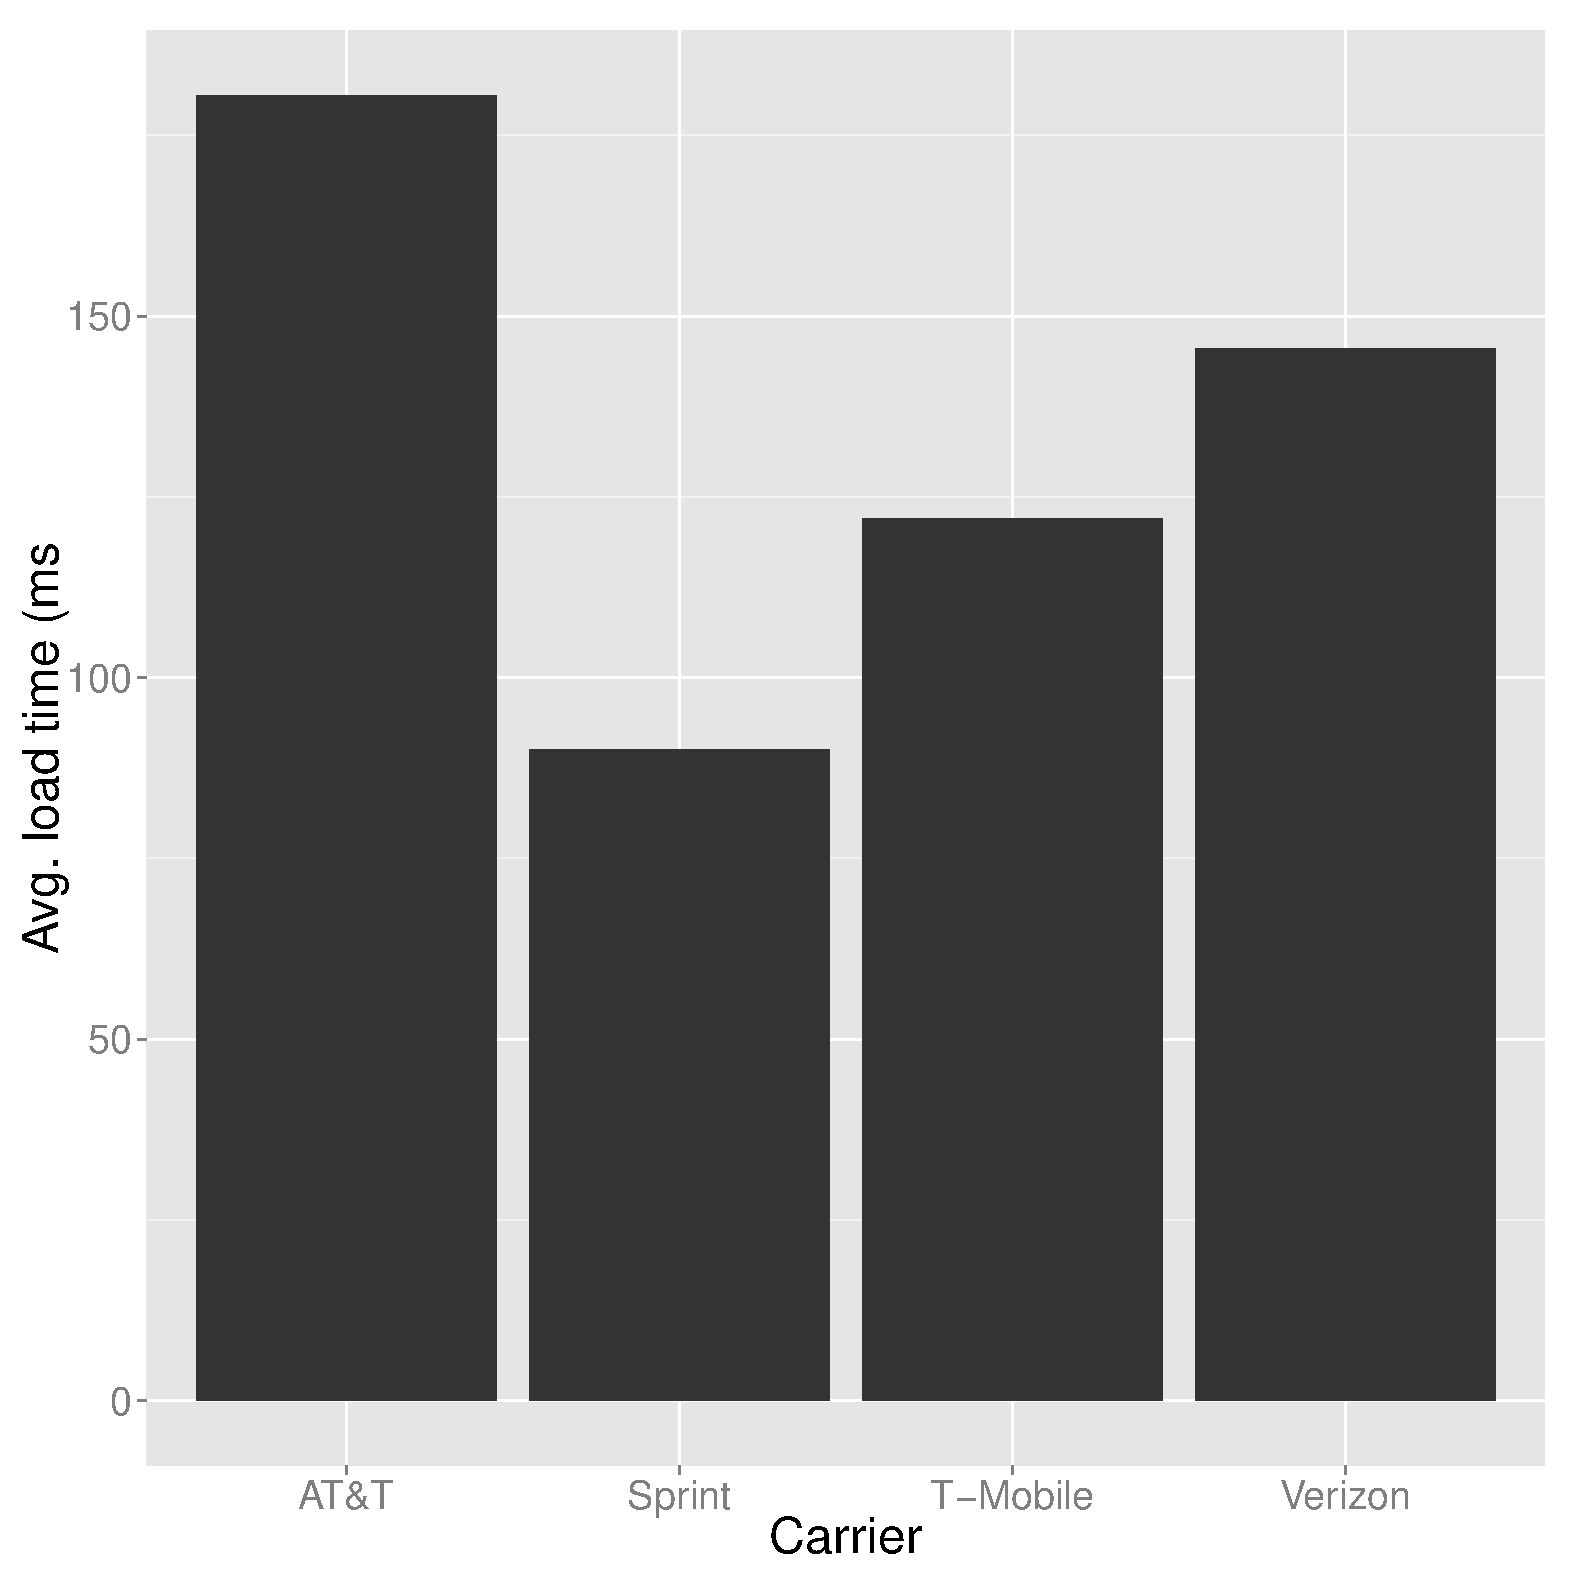
\includegraphics[width=4cm] {Images/dist1.pdf}}
% 		\caption{Visualization: Average \\ Load Times by Carrier
% 		 for BadApp}
% 		\label{fig:staplerX}
% 	\end{subfigure}
	
% 	\centering
% 	\begin{subfigure}{0.49\linewidth}
% 		{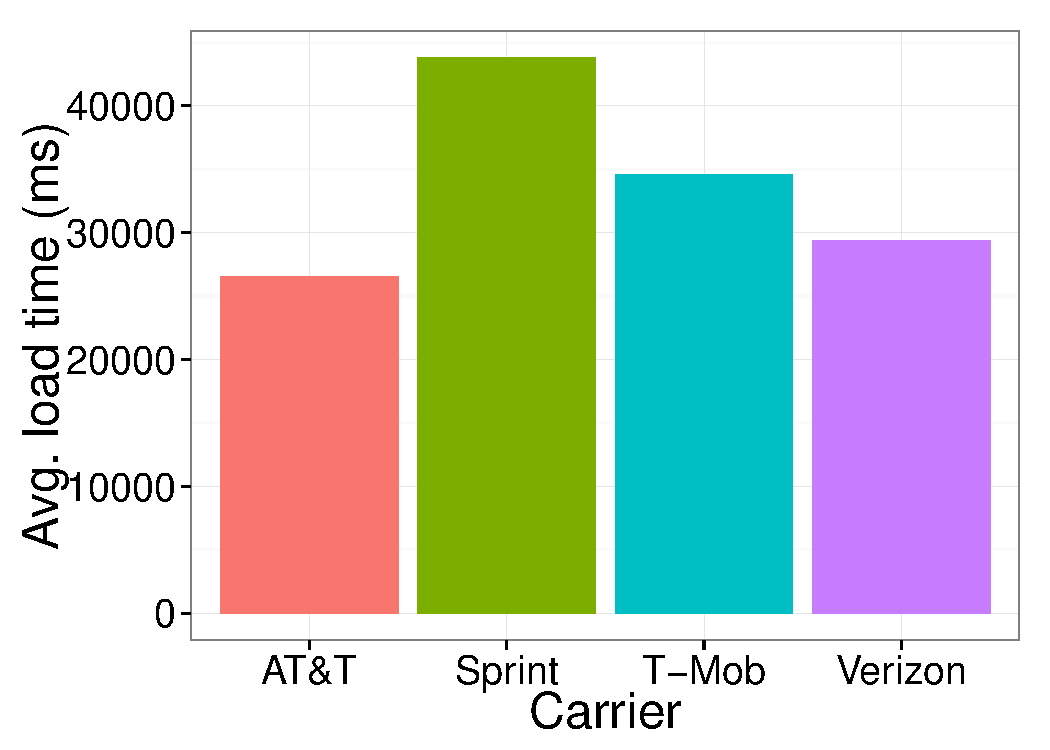
\includegraphics[width=4cm] {Images/dist2.pdf}}
% 		\caption{Scenario A: Average Load Times by Carrier}
% 		\label{fig:staplerX-a}
% 	\end{subfigure}
% 	\begin{subfigure}{0.49\linewidth}
% 		\centering
% 		{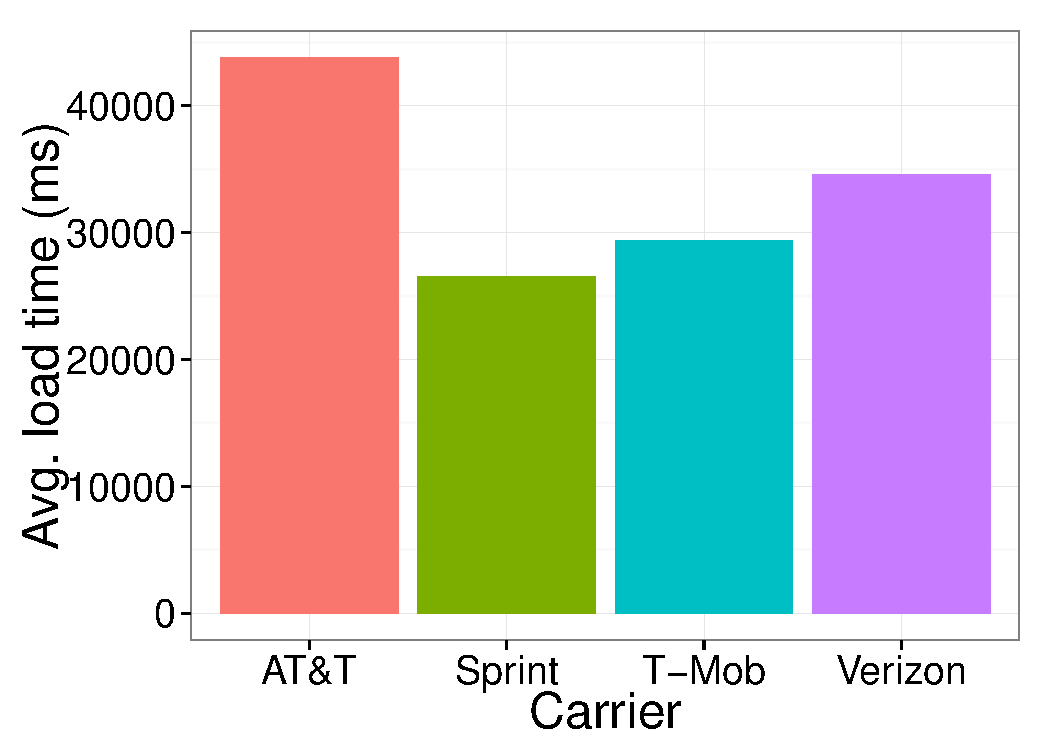
\includegraphics[width=4cm] {Images/dist3.pdf}}
% 		\caption{Scenario B: Average Load Times by Carrier}
% 		\label{fig:staplerX-b}
% 	\end{subfigure}
% 	\vspace{-10pt}
% 	\caption{Motivating Example}
% 	\label{fig:intro}
% 	\vspace{-15pt}
% \end{figure}

%%%%%% VLDB original end %%%%%%%

\reviewer {
	W2: Using the illustrative example is helpful, but would have been even more
helpful if it would be based on a real dataset actually used in the evaluations. 
Using the illustrative example was helpful and quite motivating.
However, this introduced another dataset not used in the evaluations
afterwards. To use a dataset, which was actually used in the evaluation would
make the presentation more coherent. Figure 1 uses the BadApp dataset,
Figure 3 a donation dataset, then other datasets are introduced for the
evaluation, and the diabetes dataset for the user studies. Focusing on the
diabetes dataset in Figure 1 and Figure 3 would leave more room to reuse
them to discuss some findings for example using Figure 3.
}
\mpv{sure, if we have time} \agp{I think this is worth investing 
the time in--shouldn't take more than half an hour to dig up, right? We can
also point at these visualizations and say that these were actually
returned by \SeeDB.}
\srm{I agree!}


\begin{example}
Consider a smartphone app analytics team that is tasked with answering why a certain app, 
BadApp, is showing poor performance and receiving consumer complaints. 
Suppose that the team uses the AppMetrics database containing metrics such as network usage, 
power consumption, and load times to perform the analysis.
The analyst begins by querying the AppMetrics database for BadApp-specific data and uses her 
favorite visualization software to graph various metrics for BadApp.

For instance, she may visualize average network usage for BadApp, 
correlation between session times and number of crashes, average load times by carrier, 
comparison of mobile operating systems running BadApp vs.~other apps, and so on,
in order to identify what metrics BadApp may be misbehaving on.
Depending on the types of visualizations created, the number of possible 
visualizations grows exponentially with the number of metrics in the database,
such that creating and examining all possible visualizations
becomes untenable.
% For example, the visualization for average load times by carrier is generated by running an operation equivalent to the
% SQL query (Q') shown below.
% %The result of this query is a two-column table that is very likely going to be viewed as a bar-char~\cite{vql, kristi}.
% Table \ref{tab:staplerX} and Figure \ref{fig:staplerX} respectively show an example of the results of Q' and a potential
% visualization.

% \noindent
% \begin{align*}
% & \tt Q' = SELECT \ \ carrier,\ AVG(load\_time) \ \ FROM \ \  AppMetrics \\
% & \tt \hspace{20pt} WHERE\ Name=``BadApp" \ \ GROUP  \ \ BY \ \ carrier
% \end{align*}



\begin{figure}[h]
\vspace{-10pt}
	\centering
	\begin{subfigure}{0.49\linewidth}
	   \begin{tabular}{cc} \hline
		  Carrier & Load Times (ms) \\ \hline
		  AT\&T & 180.55 \\ \hline
		  Sprint & 90.13 \\ \hline
		  T-Mobile & 122.00 \\ \hline
		  Verizon &  145.50\\ \hline
		  \end{tabular}
		  \caption{Data: Average Load Times by Carrier for BadApp} \label{tab:staplerX}
	\end{subfigure}
	\begin{subfigure}{0.49\linewidth}
		\centering
		{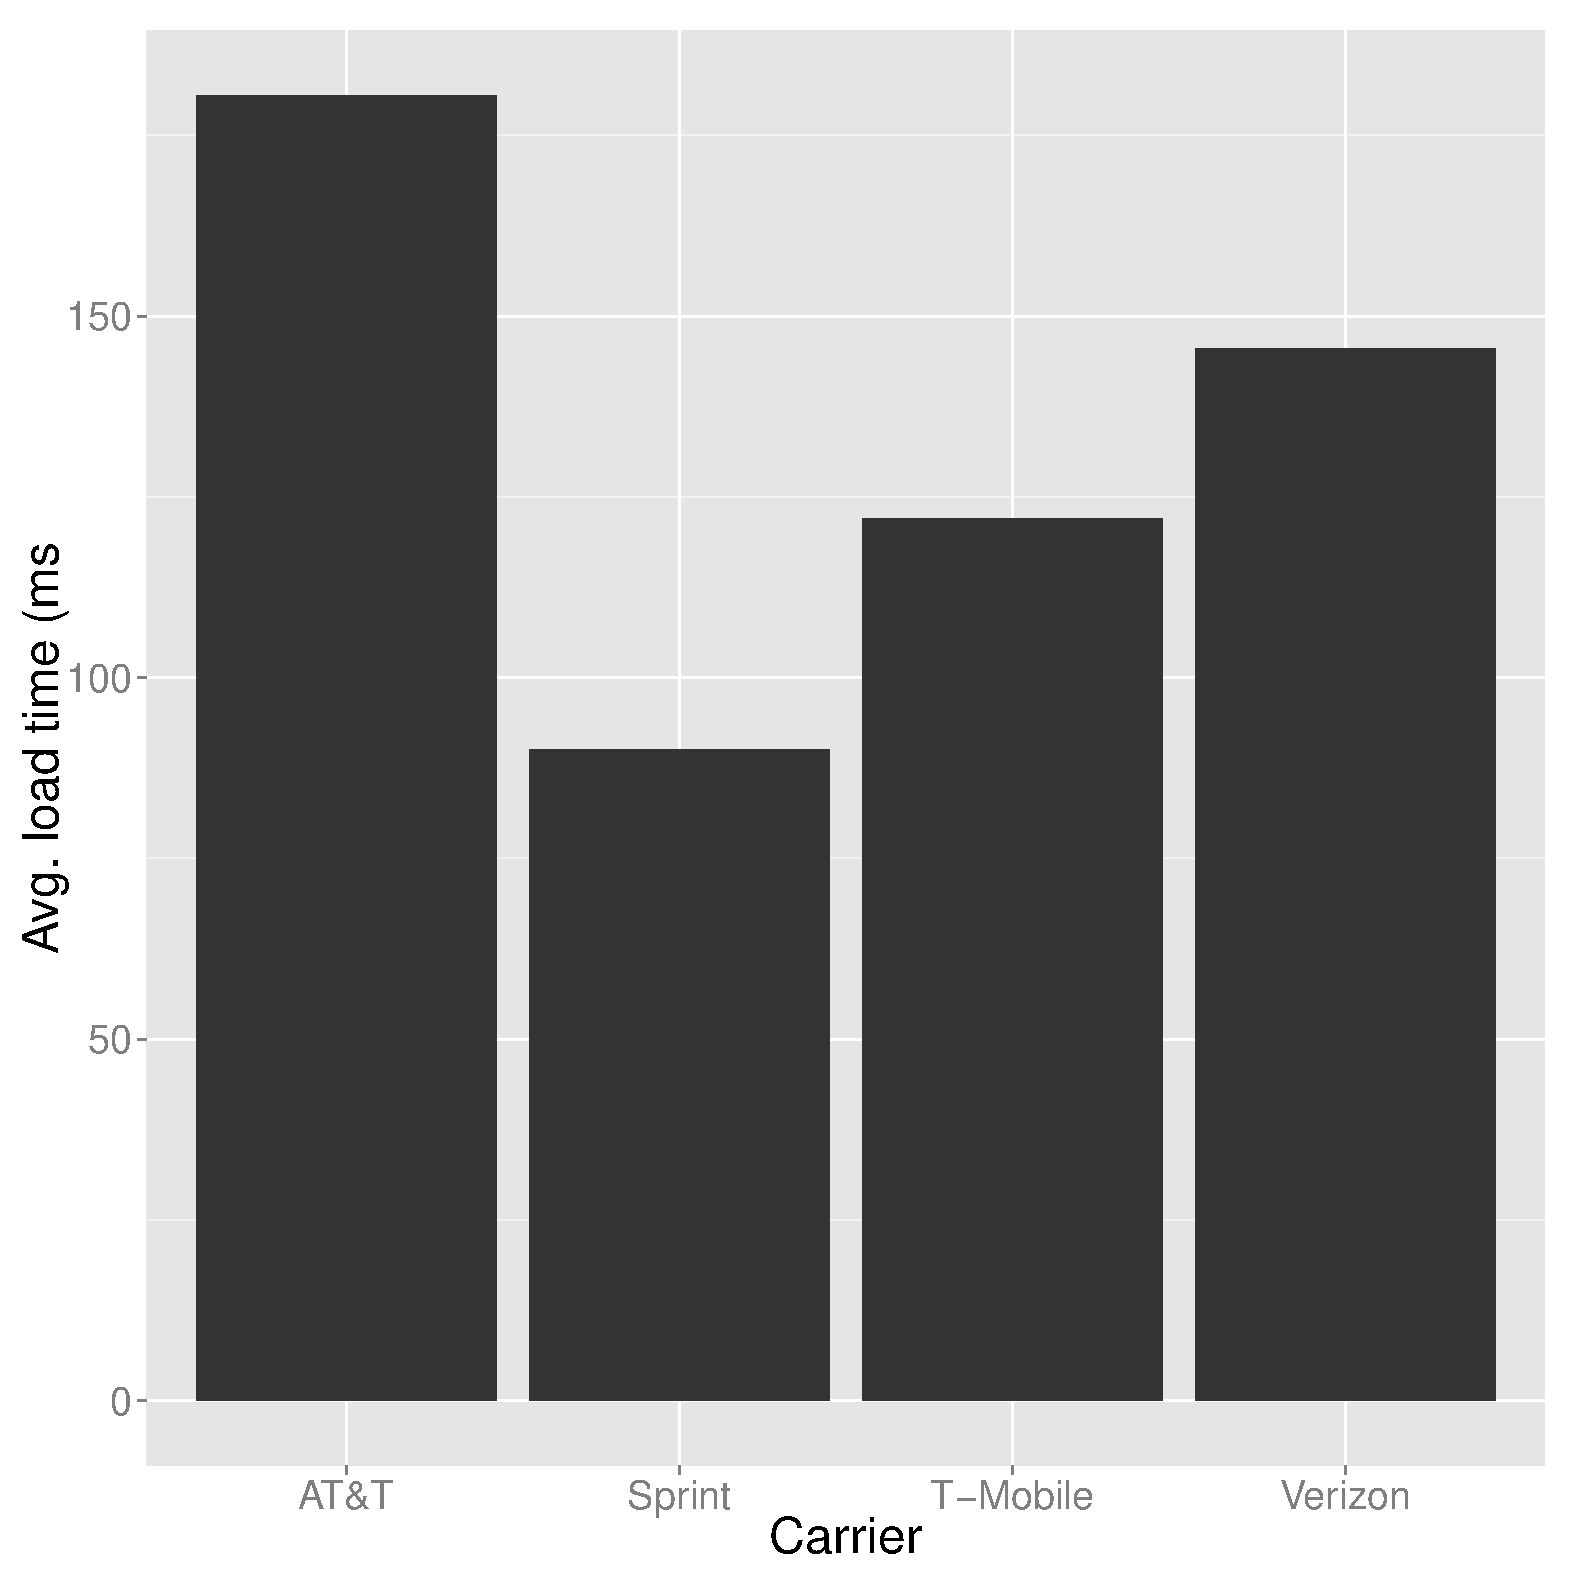
\includegraphics[width=4cm] {Images/dist1.pdf}}
		\caption{Visualization: Average \\ Load Times by Carrier
		 for BadApp}
		\label{fig:staplerX}
	\end{subfigure}
	
	\centering
	\begin{subfigure}{0.49\linewidth}
		{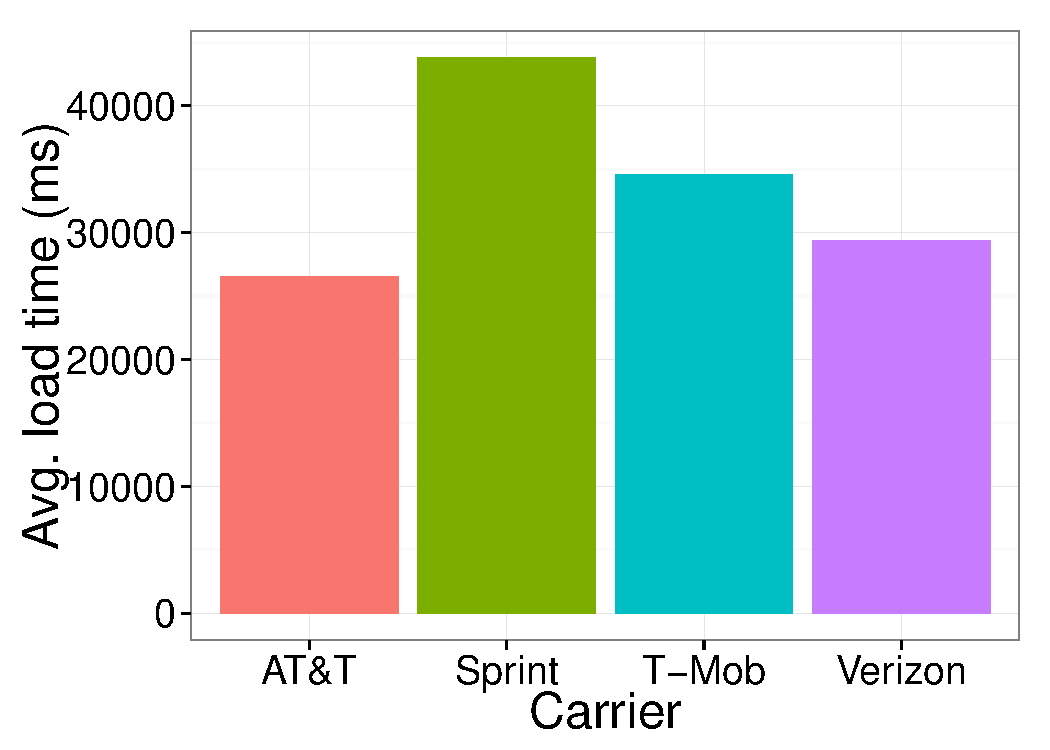
\includegraphics[width=4cm] {Images/dist2.pdf}}
		\caption{Scenario A: Average Load Times by Carrier}
		\label{fig:staplerX-a}
	\end{subfigure}
	\begin{subfigure}{0.49\linewidth}
		\centering
		{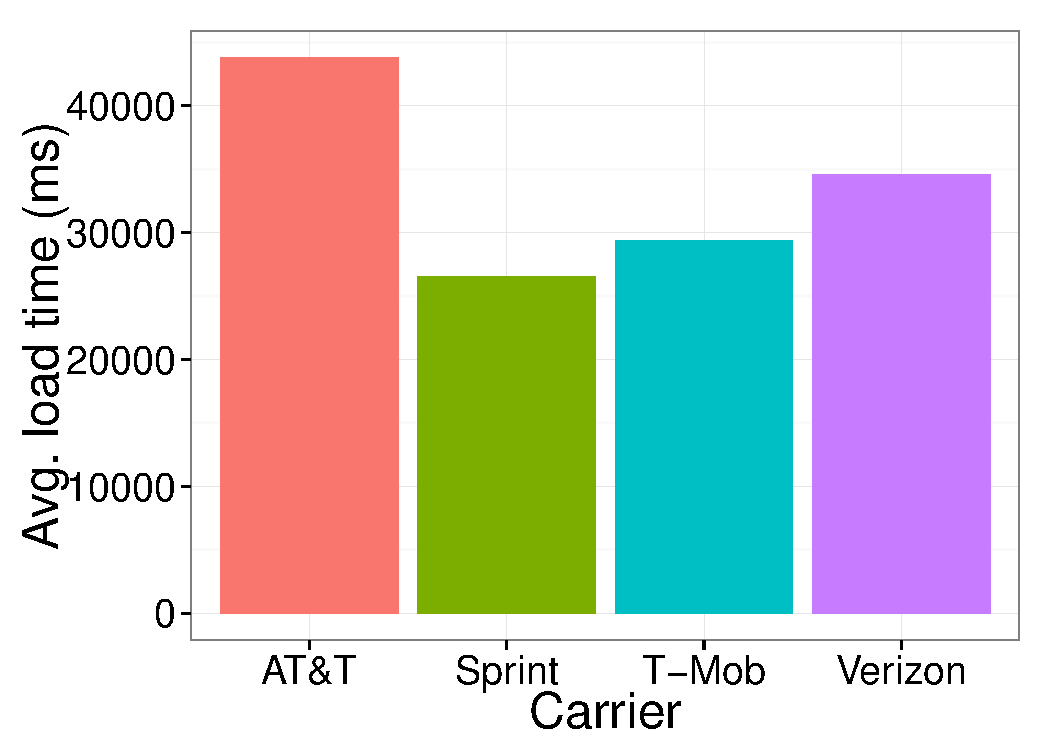
\includegraphics[width=4cm] {Images/dist3.pdf}}
		\caption{Scenario B: Average Load Times by Carrier}
		\label{fig:staplerX-b}
	\end{subfigure}
	\vspace{-10pt}
	\caption{Motivating Example}
	\label{fig:intro}
	\vspace{-15pt}
\end{figure}

%What might make one of these visualizations ``interesting'' or valuable for the 
%task at hand depends on a number of factors.
\srm{I suggested below that our user studies show that users like our metric. Do we believe this?}\agp{rewrote to remove preference}
As noted above, we have identified that 
analysts find visualizations that show
cases where the data deviates from some underlying distribution to be interesting.
In the case of app analytics, this underlying distribution might be metrics for
all apps, versus the distribution of particular metrics specifically in BadApp.
As an example, our user studies suggest that users will find the visualization of load times by carrier (Figure
\ref{fig:staplerX}) more interesting if the trend for load times across all
apps shows the {\it opposite} trend (e.g. Figure \ref{fig:staplerX-a}), and less interesting if the overall trend for all apps followed a similar trend.
(Figure \ref{fig:staplerX-b}).  
\end{example}



\mpv{acknowledge that this is from the vision paper?} \agp{Not necessary}

\mpv{Say that metric is suited to when there user is unfamiliar with the data, cold
starts?}
\agp{We need to articulate that our goal is to build \SeeDB that actually makes
these recommendations.}
%Since our goal with \SeeDB is to make visual analytics faster, we adopt a metric
%that prefers visualizations that show interesting or surprising trends in data.
%Specifically, we are motivated by the following observation:
%\begin{quotation}
%The greatest value of a picture is when it forces us to notice what we never expected to see.
%\end{quotation} 
%\begin{flushright} 
%- John Tukey, Exploratory Data Analysis 1977
%\end{flushright}

% While this utility metric is an example of a simple recommendation metric,
% it plays an important role in recommendations when 
% there is no prior history --- and therefore no user preferences
% or understanding of context.
% This special case is especially appropriate when the analyst
% is not very familiar with a dataset and is analyzing it for the first time.
% That said, in Section~\ref{sec:discussion}, we describe how our deviation-based
% metric can, in fact, encompass a large number of data-driven utility metrics and
% can be seamlessly extended to support other dimensions such as user preferences.

\srm{the following is substantially edited / cut back.}
We formally define the deviation-based scoring function in the next
section.  As noted above, in addition to our deviation-based metric,
there are of course many other dimensions (aesthetics, user
preferences, etc.) that can influence the perceived utility of a
visualization a few of which we discuss in Section
\ref{sec:discussion}, leaving a detailed investigation of such metrics
for future work.


%These include other functions based on data distribution (e.g. scoring based on 
%statistical summaries) and functions that measure utility along {\em 
%dimensions} other than data distribution. 
%These utility dimensions 
%include aesthetics (e.g. is a bar plot more appropriate than a 
%scatter plot), context (e.g. prior knowledge that only female patients visit the
%obstetrics department), and user preference (e.g. in the sales dataset, profit is
%the most relevant attribute).
%Exploration of each of these dimensions forms a distinct body of work.

% functions 
% that can be used to score the utility of a 
% visualization; these can be different functions based on data distribution (e.g. scoring
% based on statistical summaries of data or outlier detection) or functions that take
% orthogonal {\em dimensions} of utility into account, e.g., user preferences, aesthetics, and context.
% The pruning framework we propose in Section \ref{sec:in_memory_execution_engine} can be applied to a large set of 
% functions derived from data distribution, and \SeeDB
% can support these metrics without any changes. \mpv{Verify true? Add characterization
% of metrics}
% Investigations of the other dimensions of utility form a distinct body of work, and
% we leave these explorations for future work.
% \mpv{keep? In section \ref{sec:discission}, we outline some means by which \SeeDB may be 
% extended to support these metrics.}
% We leave the investigation of other dimensions of utility to future work, but outline
% in Section \ref{sec:discussion} some means by which \SeeDB may be extended to support them.

% Due to the scale of data, most common visualizations show aggregate summaries of data
% as opposed to individual records (e.g. average sales by state vs. sales of each store 
% in every state).
% Consequently, our current implementation of \SeeDB\ recommends visualizations that show aggregate 
% summaries of data.

% Of course, there are a variety of other possible data-driven metrics for quality or utility
% of a visualization.
% For instance, one might focus on visualizations that show order statistics or anomalies~\cite{DBLP:conf/avi/KandelPPHH12}. 
% These would be important for spotting, for example, unusual spikes in machine load.
% Similarly, drawing upon the literature on data cubes, one might choose visualizations that highlight aggregates that
% are unusual given the remaining values in the cube~\cite{DBLP:conf/vldb/Sarawagi00}.
% Finally, one might choose to not aggregate any values but show correlations between attributes by plotting a random
% sampling of data-points.  Incorporating these other types of visualizations into our framework is an interesting
% direction for future work.

\reviewer{
	The method does not consider the context, semantics, and any user
preferences all important components of viz	
}
\mpv{Yeah I say that above. Any additions?}



% The majority of visualizations that are generated in visualization systems are based on aggregate summaries of the
% underlying data.
% As a result, the {\it trends} we study are the results of grouping and aggregation applied to a given dataset.


% Thus, the recommendation algorithm used by \SeeDB\ works as follows: given a dataset $D$ and a query $Q$
% indicating the subset of data of interest to the analyst, \SeeDB finds the visualizations of $Q$ that 
% show the highest deviation between trends in $Q$ and trends in $D$. 
% Specifically, \SeeDB considers visualizations that can be constructed via a combinations of grouping and 
% aggregation applied to $Q$.

No existing system is that we are aware of makes use of variation in the underlying
data to recommend visualizations.  
Current visualization packages like Spotfire~\cite{Ahlberg:1996:SIE:245882.245893} and Tableau~\cite{tableau,polaris} have limited capabilities for 
recommending visualizations.
Their recommendations only implement rules-of-thumb 
regarding chart aesthetics such as choice of
chart type, colors and marks, borrowed from
classical work by Mackinlay~\cite{Mackinlay:1986:ADG:22949.22950} and Cleveland and Gill~\cite{cleveland1984graphical}.
%No existing system that we are aware of leverages insights about the underlying data
%into make visualization recommendations. \mpv{does this sound ok?} \agp{I would start with
%the statement that no current system supports the recommending of interesting visualizations
%where the target dataset shows some discrepancies not found in the underlying data.
%Then say the first two lines.}


Our system, \SeeDB, is built as a middleware layer that can run on any 
relational database system (row or column store), 
seamlessly benefiting from optimizations to 
the database. 
In this paper, we develop and validate the use of  
two orthogonal techniques to make tractable the problem
of recommending visualizations based on deviation:
\begin{denselist}
\item {\em Sharing Computation.} 
We develop a suite of multi-query optimization techniques to share computation
among the candidate visualizations,
reducing time taken by ?X. \agp{fill in.}
\item {\em Pruning Computation.}
We develop a pruning technique to avoid wasting computation
on obviously low-utility visualizations, adapting
techniques from traditional 
  confidence-interval-based~\cite{hoeffding1963probability} 
  top-$k$ ranking and the
  multi-armed bandit~\cite{bandits},
  further reducing time taken by ?X. \agp{fill in.}
\end{denselist}
Lastly, we develop a general {\em phase-based execution framework}
that allows us to leverage the benefits of these two techniques
in tandem, reducing the time for execution by over ?X,
making recommendations feasible in real-time. \agp{fill in}

We present the experimental evaluation of \SeeDB 
via both a performance study and a user study.
In summary, the contributions of this paper are:

% efficiently manages the search
% for data-driven visualization recommendations at interactive time scales.
% We show that \SeeDB can be implemented on top of a traditional relational database,
% allowing it to take advantage of the benefits of the interfaces and features
% relation engines expose.
% Doing this, however,
% also leads to inefficiencies that arise due to the requirement that data be
% accessed via SQL.   
% We manage these inefficiencies by introducing two classes of optimizations:
% {\em sharing-based} optimizations, that try to batch
% and share as much computation as possible to minimize the number of SQL queries,
% and {\em pruning-based optimizations}, that try to avoid
% as much unnecessary work as possible, and discarding candidate aggregate views
% that are of low utility.

\mpv{revisit contributions} \agp{The order of this is off.}
\begin{denselist}
%  \item We design \SeeDB as a system for data-driven visualization recommendations.
%  We explore and evaluate two distinct implementations of the system, one as a
%  wrapper around a database and another a custom solution (Section~\ref{sec:system_architecture}).
  \item We present \SeeDB, a visualization recommendation system that can run
  as a middleware layer on any SQL-compliant DBMS (Section~\ref{sec:system_architecture}).
  \item We adopt and evaluate a deviation-based scoring function for measuring utility
  of a visualization (Section~\ref{sec:problem_statement}).
  \item We propose a set of multi-query optimization techniques which in combination
  with the pruning framework maximize the sharing of computation between visualization
  computations (Section~\ref{sec:sharing_opt}).
  \item We propose a general-purpose view pruning framework to quickly identify
  high-utility visualizations by adapting techniques from traditional 
  confidence-interval-based~\cite{hoeffding1963probability} top-$k$ ranking and the
   multi-armed bandit problem~\cite{bandits} (Section~\ref{sec:in_memory_execution_engine}).
  % \item We describe a general deviation-based framework 
  % for evaluating the utility  of a visualization,
  % and present and evaluate a specific metric that identifies 
  % aggregate dimensions in a dataset that
  % show maximal variation (Section~\ref{sec:problem_statement}).
  % We develop two classes of optimizations to make such aggregates run fast 
  % in a conventional DBMS.
  % \item The first set of techniques
  % combine queries and aggregates to minimize the number of queries executed and 
  % maximize the sharing of scans between queries, 
  % including bin-packing~\cite{garey} algorithms and parallelization
  % (Section~\ref{sec:sharing_opt}).
  % \item The second set of techniques further optimize the process by adapting techniques 
  % from both traditional confidence-interval-based~\cite{hoeffding1963probability} top-$k$ ranking and the
  %  multi-armed bandit problem~\cite{bandits} 
  %  to the problem finding the top-$k$ visualizations (Section~\ref{sec:in_memory_execution_engine}).
  % \item We explore visualization pruning techniques based on data distribution
  % to prune visualizations even before they are evaluated by the \SeeDB\ system 
  % (Section~\ref{sec:pruning}).
  \item We evaluate the performance of our pruning framework and demonstrate that \SeeDB
  can identify high-utility visualizations with high accuracy. We also demonstrate that 
  our optimizations provide a 40-100X speedup on both relational row and column stores
  (Section~\ref{sec:experiments}). 
  \item We present the results of a user study evaluating the role of visualization 
  recommendations in visual analysis and the quality of \SeeDB recommendations in particular
  (Section \ref{sec:user_study}), showing that our deviation-based metric is able to yield visualizations that users find interesting.
\end{denselist}

\noindent Finally we note that the vision for \SeeDB\ was described in a vision paper~\cite{DBLP:conf/vldb/Parameswaran2013} and presented as demonstration~\cite{DBLP:journals/pvldb/VartakMPP14}, but neither of these short papers described detailed algorithms or
presented any form of evaluation.
Specifically, this work builds upon the \SeeDB vision by proposing a novel, general-purpose view 
pruning framework, a combination of multi-query optimization techniques, and presenting 
both a performance study of the system as well as a user study demonstrating the efficacy of our system in aiding analysis.
\reviewer{
	I like the ideas in this paper, but they have been presented in a vision paper
and demo paper. So to warrant a new publication the execution of these
ideas (the specific search techniques) and their evaluation need to be novel,
interesting, and well executed. I found the evaluation in particular to be
lacking.
}

\reviewer{
	This paper’s contribution seems to be mostly section 4.3 (pruning
optimizations) and the tests (Sections 5 and 6). The differences with
references [27] and [37] should be made more clear.
}



%!TEX root=document.tex
\section{Problem Statement}
\label{sec:problem_statement}
\resolved{
\srm{This rewrite is good, thanks Aditya!}
\srm{We need to define what measure and dimension attributes mean;
in a snowflake schema a dimension attribute would be anything in a dimension table, and a measure attribute would be a non-foreign
key column in a fact table. I don't think that's what we mean.  I think these are actually properties of the query, right, i.e., 
dimension attributes are those appearing in the group by clause?  We should use different names.}\agp{I've addressed this somewhat.}
}
As is standard in OLAP, and in visual analytics
tools such as Tableau and Polaris~\cite{tableau,polaris},
we focus on a database $D$ with a snowflake schema.
We denote the attributes
that we would like to group-by in our visualizations 
as {\em dimension attributes}, $A$, and 
the attributes that we would like to 
aggregate in our visualizations
as {\em measure attributes}, $M$.
Further, we denote by $F$ the set of potential
aggregate functions over the measure attributes (e.g. COUNT, SUM, AVG).  
For visualization purposes, we assume that we can group $D$ along any of the dimension attributes $A$ 
and we can aggregate any of the measure attributes $M$.
This leads to a two-column table that can be easily visualized
via standard visualization mechanisms, such as bar charts or trend lines.
(Recent work has shown that bar charts are the overwhelming majority of visualizations
created using visual analytics tools~\cite{DBLP:journals/pvldb/MortonBGM14}.) 
Our techniques also apply to the general Polaris table algebra~\cite{polaris}, where
we can aggregate across multiple attributes at once, and group-by multiple attributes, 
potentially leading to more than two columns.
For ease of exposition, we focus on two-column result visualizations in this paper,
which can be readily visualized using bar charts or trend lines.

In addition to the database $D$, we assume that the analyst has indicated
a desire to explore a subset of data specified by a query $Q$.
The goal of \SeeDB is to recommend visualizations of $Q$ that have
high utility (which we measure using deviation, as explained below).
The class of queries $Q$ posed over $D$ that we support encompass a general class of queries 
that select a horizontal fragment of the fact table and one or more dimension tables.
Conceptually, we can view this as a simple selection query over the result of joining all
the tables involved in the snowflake schema. 
That said, we can also support projections and joins which essentially have the effect
of respectively dropping certain columns or tables from consideration in the visualizations.
Thus, we support a general class of select-project-join (SPJ) queries over the snowflake schema.
For the purpose of this discussion, we focus on simple selection
queries over the result of joining all the tables in the snowflake schema.
We note that this class of queries 
suffices for most visualization tasks.
For instance, in our illustrative example, $Q$ can select any subset of records from the
Census table. 
We denote the result of $Q$ as $D_Q$.
\resolved{
\srm{Although this notion is compact, it doesn't seem to capture
the contents of the WHERE clause.}\agp{rewritten to make clear that
it is a function.}
}

Each \SeeDB visualization  can be translated into an agg\-re\-gate / group-by
 query on the underlying data.
% Since each visualization represents an aggregate summary of the underlying data,
% the visualization can be distilled into an aggregate and grouping query.
% Borrowing from the data cube literature~\cite{olap}, 
% we call these summaries aggregate {\it views}.
% where an aggregate view
% is the result of applying grouping and aggregation to a dataset.
We represent a visualization $V_i$ 
 as a function represented by a triple $(a, m, f)$, 
where $m \in M, a \in A, f \in F$.   
We call this an {\em aggregate view} or simply a {\em view}.
The aggregate view performs a group-by on $a$ and applies the aggregation function $f$ 
to measure attribute $m$. 
As an example, $V_i(D)$ represents the results of grouping
the data in $D$ by $a$, and then aggregating the $m$ values using $f$;
$V_i(D_Q)$ represents a similar visualization applied to
the data in $D_Q$.
% While \SeeDB techniques can be used to recommend visualizations
% generated via multi-attribute grouping and aggregation,
% for simplicity, we focus on views generated by single attribute grouping. 
\resolved{
\reviewer {D1.2 I wonder what is really specific to visualizations. Indeed, a visualization
as defined by the authors seems to be a two column table (attribute,
measure). Is it usual to define visualizations this way?
}
\mpv{
	Aggregate summaries visualized as bar charts and column charts are in fact, extremely
	common visualizations, and hence are the first visualizations tackled by \SeeDB.
	The techniques we develop here are general and have possible applications 
	in traditional data mining. It would be interesting to explore these applications
	further.
}
\agp{I think we can amend the response to say it is standard (cite polaris table algebra)
to define visualizations in this manner.}
}
\if{0}
Given a database $D$ and the subset of data selected by the analyst (via query $Q$), 
the goal of \SeeDB is to recommend visualizations of $Q$ that have high utility. 
\SeeDB (currently) focuses on recommending bar charts showing aggregate views of the 
data.
This choice is motivated by the fact that bar plots are the overwhelming
majority of visualizations created using visualization tools 
\cite{DBLP:journals/sigmod_record/MortonBGKM14}.
\fi
% The most common visualizations in real workloads of Tableau and ManyEyes 
% are bar charts \cite{DBLP:journals/sigmod_record/MortonBGKM14} showing aggregate views
% of the data. 
% Furthermore, the scale of data necessitates the visualization of aggregate summaries of
% data vs. individual records (e.g. average sales by state vs. sales of each store in the
% country).
% Consequently, \SeeDB (currently) focuses on this specific type of visualization.
% Due to the scale of data, most common visualizations show aggregate summaries of data
% as opposed to individual records (e.g. average sales by state vs. sales of each store 
% in every state).
% Moreover, these summaries are visualized as bar charts and column charts in the vast
% majority of cases~\cite{kristi}.
% Consequently, our current implementation of \SeeDB focuses on recommending bar and column
% charts that visualize aggregate summaries.
% Given a database $D$, associated schema $S$, and a user query $Q$, the goal
% of \SeeDB\ is to recommend visualizations of results of $Q$ with high utility. 
% As mentioned in Section~\ref{sec:introduction}, \SeeDB\ focuses on visualizations 
% that show aggregate summaries of data.
\if{0}
Let $D$ have a snowflake schema with 
dimension attributes $A$, measure attributes $M$, and potential
aggregate functions $F$ over the measure attributes. 
%Similar to cube aggregates, 
For visualization purposes, we assume that we can group $D$ along any of the dimension attributes $A$ 
and we can aggregate any of the measure attributes $M$.
Our system currently limits the class of queries $Q$ posed over $D$ to be single-table
selection (and optionally projection) queries.
We find that simple selection queries suffice for most visualization tasks.
For instance, in our illustrative example, $Q$ can select any subset of records from the
AppMetrics table. 
Adding projections to $Q$ serves to limit the the dimension and measure 
attributes used by \SeeDB in constructing visualizations.
We denote the result of $Q$ as $D_Q$.
\fi
% dimension attributes are either nominal, ordinal, or numeric,
% but typically with a small number of distinct values;
% these are the attributes along which we can perform a group-by.
% Measure attributes are numeric attributes which take on a large number 
% of distinct values; 
% these are the ones that are typically aggregated.
% We limit the class of queries $Q$ posed over $D$ to be
% those that select one or more rows from the fact table, 
% and denote the results as $D_Q$. 
% For instance, in a product sales table, $Q$ could select
% all tuples corresponding to transactions involving bicycles.
% Given query $Q$, \SeeDB\ considers all aggregate views 
% $V_i$ obtained by performing a grouping and aggregation on $D_Q$. 
\resolved{
\reviewer{The range of queries that are supported is not clear. Specially in fig.3, in
the ``SQL'' tab, it seems that users can only define very simple selection
queries (where the selection is a simple conjunction of predicates). No
project, no joins, no difference, no grouping/agg. Is this correct? Why call
this SQL?}
\mpv{New interface only allows selections}
\agp{I don't think we should restrict ourselves to selection. We can
support SPJ queries over the snowflake schema.}
}
\resolved{
\reviewer {
	D2.1 The approach seems limited to simple queries of the form Select * from
aTable where someSelectionPredicates. It seems to me that it is quite a
limitation in the sense that the authors implicitly position their work in a data
warehouse exploration context (as per Section 2). I would like the authors to
comment that point. For instance, what about when the projection is not
select * but select aListOfAttributes?
}
\mpv{Do we need to defend why we support only simple queries? From other studies of
visualization tools, a significant portion of queries posed in these tools is 
limited to simple selection and projection tasks ~\cite{}.
Therefore, we have prioritized support for operations over more complex queries.}
\agp{I think we can clarify this in the response, but see what I've said above.}
}
\resolved{
\reviewer {
	D2.2 In the definition of $U(V_i)$: as $D_Q $contains a selection that D does not
have, how to ensure that the population of the two distribution is the same?
}
\mpv{
	This should only be in the reviewer response: the dataset under study $D_Q$ can be
	compared to various {\em comparison} datasets; by default, the comparison dataset
	is set to the full dataset $D$ (to observe overall trends), but can be set to any 
	other subset of data.
	Depending on the analytical task, one may want the two populations to be similar 
	(males and females in a given age group) or different (comparison of young adults to seniors). 
	Since the system has limited knowedlge about the exact analytical task, we provide 
	users with flexiblity to choose a comparison dataset.
}
}
% Note that all such $V_i$ give rise to two-column results that can 
% be readily visualized (e.g. Table~\ref{tab:staplerX}). 
% Consider a database $D$, and associated metadata $M(D)$, with a snowflake schema,
% with dimension attributes $A$, measure attributes $M$, and potential
% aggregate functions $F$ over the measure attributes.
% Dimension attributes are either nominal, ordinal, or numeric,
% but typically with a small number of distinct values;
% these are the attributes along which we can perform a group-by.
% Measure attributes are numeric attributes which take on a large number 
% of distinct values; 
% these are the ones that are typically aggregated.

% Given a database $D$ and a query $Q$, \SeeDB\ considers a number of views (i.e., aggregate queries) that
% can be generated from $Q$ by adding relational operators.
% For the purposes of this discussion, we will refer to views and visualizations
% interchangeably, since it is straightforward to translate views into
% visualizations automatically~\cite{DBLP:journals/cacm/StolteTH08}. 
% For example, there are straightforward rules that
% dictate how the view in Table~\ref{tab:staplerX} can be transformed to give a
% visualization like Figure~\ref{fig:staplerX}.

% For this work, we classify attributes of a table into
% two types: {\it dimension attributes} and {\it measure attributes}. 
% Dimension
% attributes are attributes that are nominal, ordinal or numeric but with a small
% number of distinct values. 
% These are the attributes along which we can perform a group-by. 
% Measure attributes on the other hand are numeric attributes will a
% large number of distinct values. 
% We consider views where the dimension attributes are
% aggregated with respect to these measure attributes.
%Lastly, for simplicity, 
%we ignore {\em binning}: that is, given a view to be visualized,
%there are many ways of binning values to give the view. 
%For instance, if we have average profits per day, we can bin the days into
%months, into weeks, or into years.
%  aggregate view $V_i$ by
% comparing data distribution in the query results to the data distribution of the underlying dataset.
% taking into consideration a variety of aspects, including
% user preferences, metadata, query data, background data, and context.
% For now, and for most of the paper, however, 
% That said, our techniques also seamlessly apply to a more general 
% class of distance metrics described in .
\SeeDB determines the utility of 
visualizations via deviation; visualizations that show different trends in the query
dataset (i.e. $D_Q$) compared to a reference dataset (called $D_R$) are said to have high
utility.
The reference dataset $D_R$ may be defined as the entire underlying dataset ($D$),
the complement of $D_Q$ ($D$ - $D_Q$) or data selected by any arbitrary query $Q'$ ($D_{Q'}$).
The analyst has the option of specifying $D_R$; we use $D_R = D$ as the default if the analyst does not specify a reference. 
% We discuss in Section~\ref{sec:other_utility_metrics} how other distance metrics can be 
% incorporated into our system without any changes. 
Given a view $V_i$, the deviation-based utility of $V_i$ is
computed as the deviation between the results of applying $V_i$ to the query data, $D_Q$,
and applying $V_i$ to the reference data, $D_R$.
View $V_i$ applied to the results of $Q$ can be expressed as query $Q_T$ below. 
We call this the {\em target view}.
$$ Q_T\ =\ {\tt SELECT \ } a, f(m) \ \ {\tt FROM} \  D_Q\  {\tt GROUP \ \ BY} \ a$$ 
Similarly, view $V_i$ applied to the reference data $V_i (D_R)$ can be expressed as $Q_R$. 
We call this the {\em reference view}. 
$$ Q_R\ =\ {\tt SELECT \ } a, f(m) \ \ {\tt FROM} \  D_R\  {\tt GROUP \ \ BY} \ a$$
The (two) SQL queries corresponding to each view are referred to as {\em view queries}.
The results of the above view queries are summaries with two columns, namely $a$ and
$f(m)$. 
To ensure that all aggregate summaries have the same scale, we normalize each 
summary into a probability distribution (i.e. the values of $f(m)$ sum to $1$).
% over the various values of $a$ and the tables can be normalized into
%probability distributions for comparison. To convert each result table 
For our example visualization of {\em Average Capital Gain vs. Sex} (Figure \ref{fig:intro}),
the probability distribution for the target view $V_i(D_Q)$ ({\em unmarried} adults), 
denoted as $P[V_i (D_Q)]$ is: 
(F: 0.52, M: 0.48) while that for the reference view $V_i(D_R)$ ({\em married} adults), 
denoted as $P[V_i (D_R)]$ is:
(F: 0.31, M: 0.69). 
In contrast, the distributions for the visualization {\em Average Age
vs. Sex} are (F: 0.5, M: 0.5) and (F: 0.51, M: 0.49) 
for the target and reference view respectively.
Qualitatively, we see that the distributions show a large deviation for
the former visualization and hardly any deviation for the latter.

Given an aggregate view $V_i$ and probability distributions for the
target view  ($P[V_i (D_Q)]$) and reference view ($P[V_i (D_R)]$), we
define the {\em utility} of $V_i$ as the distance between these two probability
distributions. The higher the distance between the two distributions, the more 
likely the
visualization is to be interesting and therefore higher the utility.
Formally, if $S$ is a distance function,
$$ U (V_i) = S ( P[V_i (D_Q)], P[V_i (D_R)] )$$
% The utility of a view is our measure for whether the target view is
% ``potentially interesting'' as compared to the comparison view:
% the higher the utility, the more the deviation
% from the comparison view, and the more likely the associated visualization is to be interesting.
Computing distance between probability distributions has
been well studied in the literature, and \SeeDB\ supports a variety of distance
functions
to compute utility, including Earth Movers Distance, 
Euclidean Distance, Kullback-Leibler Divergence (K-L
divergence), and Jenson-Shannon
Distance. 
Our experiments use Earth Movers Distance as the default distance function,
but in Section \ref{sec:discussion} we discuss results for
other distance functions. 
Also in Section~\ref{sec:discussion}, we describe how our utility metric
can be generalized to capture other aspects of interest to analysts (beyond deviation).

We can formally state the \SeeDB problem as follows:
% Computing distance between probability distributions has
% been well studied, and \SeeDB\ supports a variety of metrics including
% to compute this distance.

% The metric may be supplied by the user, with their
% application in mind.
% Our current prototypes have the following in-built metrics
% to compute utility:
% \begin{denselist}
%   \item {\bf Earth Movers Distance (EMD)}~\cite{wikipedia-prob-dist}: Commonly used to
%   measure differences between color histograms from images, EMD is a popular metric for comparing
%   discrete distributions. This is the default metric used in \SeeDB.
%   \item {\bf Euclidean Distance}: The L2 norm or
%   Euclidean distance considers the two distributions to be points in a high
%   dimensional space and measures the distance between them.
%   \item {\bf Kullback-Leibler Divergence}(K-L divergence)~\cite{wikipedia-KL}:
%   K-L divergence measures the information lost when one probability distribution is used to approximate
%   the other one.
%   \item {\bf Jenson-Shannon Distance}~\cite{wikipedia-JS,entropy-vis}: Based on
%   the K-L divergence, this distance measures the similarity between two probability distributions.
% \end{denselist}
% Finally, we note that while other definitions of the comparison views and
% utility metrics are possible, for our initial exploration into 
% visualization recommendations, we chose to focus on the intuitive definitions above.
% In Appendix~\ref{sec:example-viz}, we perform a qualitative study of the EMD
% metric showing that it returns interesting results on real-world datasets.
% \mpv{Choice of metric should have been explained by this point}

% While we set the default \SeeDB\ distance metric as EMD (due to its simplicity),
% users can choose to use any of the distance metrics defined above. We note that
% the above definition of a view and its utility is merely one of many possible
% definitions and we choose this particular definition for simplicity and its
% intuitive nature. 
\begin{problem}
\vspace{-5pt}
Given a user-specified query $Q$ on a database $D$, a reference dataset $D_R$, 
a utility function $U$ as defined
above, and a positive integer $k$, find $k$ aggregate views $V \equiv (a, m, f)$ that
have the largest values of $U(V)$ among all the views $(a, m, f)$, 
while minimizing total computation time.
\vspace{-5pt}
\end{problem}
% Thus, \SeeDB\ aims to find the $k$ views (obtained by adding a single aggregate
% and group-by operator) that have the largest utility based on the function $U$.

% While the problem definition above assumes that we have been provided with a
% query $Q$ and we compare views on $Q$ with corresponding views on the entire
% database $D$, the \SeeDB\ framework is agnostic to where the comparison
% dataset is coming from and its contents. So the same formulation works for Use
% Cases II and III discussed in Section \ref{sec:introduction}. 





%Trend in the subset of the data that deviates from the corresponding trend in
%the overall data.
%!TEX root=document.tex

\section{{\large \SeeDB} Front-End \& Architecture}
\label{sec:system_architecture}

%In this section, we present an overview of the \SeeDB\ architecture.
% Given an input query on a dataset, the goal of \SeeDB is to recommend
% visualizations the analyst would find most valuable.
% \SeeDB recommends visualizations that the analyst would find most valuable,
% taking into account aspects such as the background, user preferences,
% and context (as discussed in Section~\ref{sec:general-metric}).

We now describe \SeeDB's front-end user experience, and then
describe the architecture and the execution engine in more detail.

\stitle{Front-end Experience.} 
We packaged \SeeDB as a recommendation plugin that can
be incorporated into a visualization tool such as Tableau or Spotfire. 
For evaluating our system, we have combined \SeeDB with a simple visualization
builder interface inspired by Polaris~\cite{polaris}.
Figure~\ref{fig:frontend1} shows the web front-end for \SeeDB 
comprising four parts 
(A) dataset selector used to connect to a database and query a specific collection of tables; 
(B) query builder used to
formulate queries using a form-based interface; 
(C) visualization builder used to manually specify visualizations; and 
(D) \SeeDB recommendations plugin 
that displays recommended visualizations.
The recommendations provided by \SeeDB change in 
response to changes in the query (B)
issued against the database.
\resolved{\srm{This is the first mention of ``human in the loop'' philosophy.  I think it might be good
to promote this to an earlier part of the paper, but only if we feel like we have something interesting
to say about it.}}
%SRM cut this -- we already said it and it doesn't really matter to VLDB reviewers
%Note that supporting basic visualization specification 
%capabilities a la Polaris, coupled with automated recommendations enabling
%the reduction of tedious manual effort,
%implies that \SeeDB will form part of a
%{\em mixed initiative}~\cite{mixed_initiative} data exploration tool.

\resolved{delete rest, too detailed:
We note that the {\em mixed-initiative} design of \SeeDB incorporating both manual
visualization specification and automated recommendations, reflects the
human-in-the-loop philosophy underlying \SeeDB.
We seek to speed up the analytics process not by completely automating the task, but
by providing the analyst real-time support while letting him or her drive the process.
}

\begin{figure}[htb]
\vspace{-15pt}
\centerline{
\hbox{\resizebox{8cm}{!}{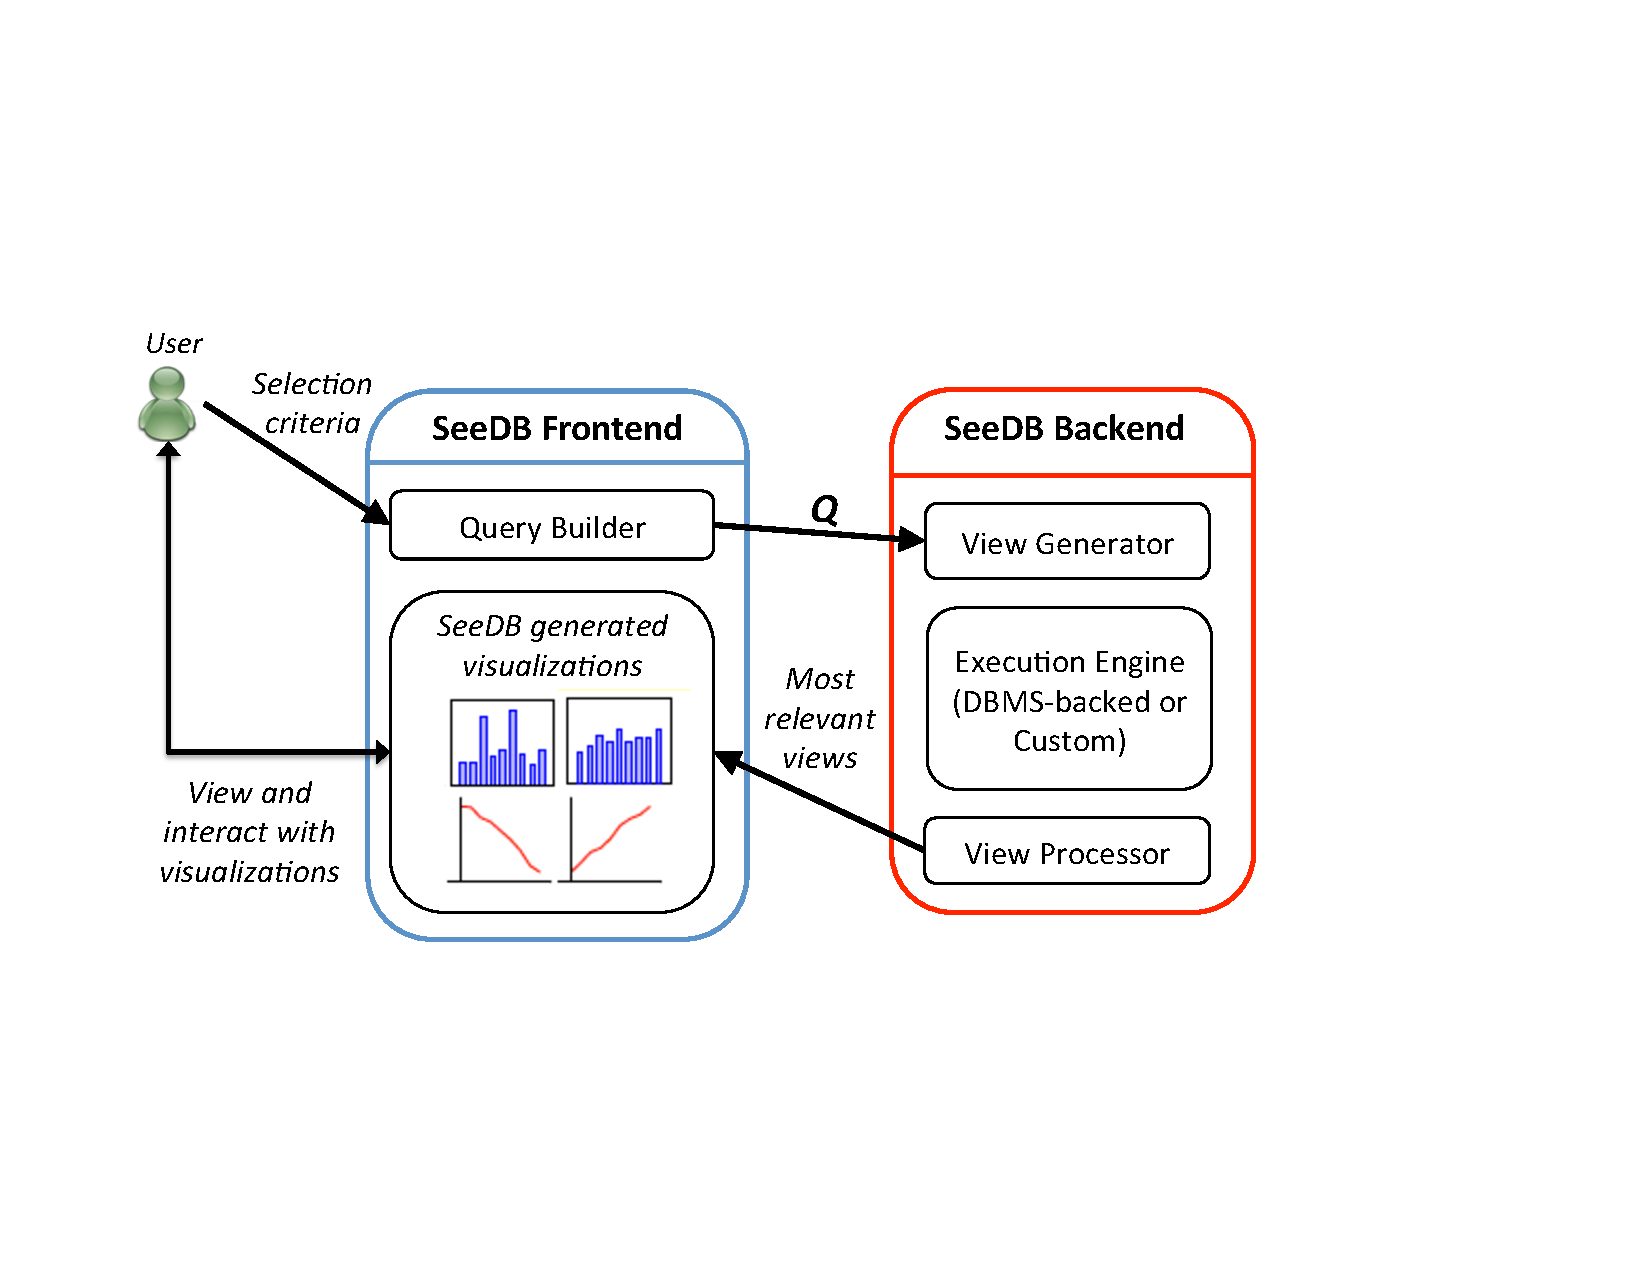
\includegraphics[trim=0 0 0 0, 
clip=true]{Images/seedb-architecture.pdf}}}}
\vspace{-12pt}
\caption{SeeDB Architecture}
\vspace{-10pt}
\label{fig:sys-arch}
\end{figure} 


\stitle{Architectural Overview.} 
\SeeDB is implemented as a middleware layer that can run on
top of any SQL-compliant database system. 
Figure \ref{fig:sys-arch} depicts the overall architecture of our
system.  The \SeeDB client is a web-based front-end that captures user
input and renders visualizations produced by the \SeeDB server.  The
\SeeDB server is composed of two main components. The first
component, the {\it view generator}, is responsible for parsing the
input query, querying system metadata and generating the list of
visualization queries that must be evaluated.  
The goal of the {\em execution engine} is to evaluate the collection of queries
 using our optimizations on top of
the underlying DBMS.
The selected aggregate views (i.e., those with high deviation) 
are sent to the \SeeDB client 
and are displayed as visualization recommendations to the user, 
who can then interact with these
visualizations.

\stitle{Basic Execution Engine.} 
To motivate the need for optimizations, we first describe 
how our execution engine would work without optimizations. 
To identify the $k$ best aggregate views,
\SeeDB needs to do the following:
For each aggregate view, it generates
a SQL query corresponding to the target
and reference view, and issues
the two queries to the underlying DBMS.
It repeats this process for each aggregate view.
As the results are received, it computes the
distance between the target and reference view
distributions, and identifies the $k$ visualizations
with highest utility. 

This basic implementation has many inefficiencies.
In a table with $a$ dimensions, $m$ measures, and $f$ aggregation functions, 
$2\times f \times a \times  m$ queries must be executed.  
As we show in Section~\ref{sec:experiments}, this can take >100s for
 large data sets.
Such latencies are unacceptable for interactive use.

\stitle{Execution Engine with Optimizations.} 
To reduce latency in 
evaluating the collection of aggregate views, 
the execution engine  
applies two kinds of optimizations:
{\em sharing}, where aggregate view queries are combined to share computation
as much as possible, and {\em pruning}, where aggregate view queries
corresponding to low utility visualizations are dropped from consideration without scanning the whole
dataset.
These optimizations are largely orthogonal to each other.
To derive benefits from both these kinds of optimizations,
we develop a {\em phased execution framework}.
Each phase operates on a subset of the dataset.
Phase $i$ of $n$ operates on the $i$th of $n$ equally-sized partitions of the dataset. 
(Empirically, we have found $n=10$ to
work well, though our results are not very sensitive to the value
of $n$.) 
For instance, if we have $100,000$ records and $10$ phases,
the $i = 4$th phase processes records $30,001$ to $40,000$.
The execution engine begins 
with the entire set of aggregate views under consideration.
\begin{denselist}
\item During phase $i$, the \SeeDB updates partial results
for the views
still under consideration using the $i$th fraction of the dataset.
The execution engine applies {\em sharing-based optimizations}
to minimize scans on this  $i$th fraction of the dataset.
\item At the end of phase $i$, the execution engine uses 
{\em pruning-based optimizations} to determine which aggregate views to discard.
The partial results of each aggregate view on the fraction from $1$ through $i$ are used to 
estimate the quality of each view, and the views with low utility are discarded. 
\end{denselist}
The retained aggregate views are then processed on the $i+1$th round,
and the process continues. 
In this manner, the set of views under consideration
decreases across these phases, with all aggregate views at the start 
of the first phase, and only the $k$ views left
at the end of the $n$th phase.
%Further, in this manner, the sharing and pruning based optimizations do
%not interfere with each other---one is applied during the phase,
%and one is applied at the end of the phase.
\papertext{The pseudocode for the phase based execution framework
can be found in the technical report~\cite{seedb-tr}.}

%We next describe the \SeeDB optimizations,
%specifically, the sharing based optimizations in Section~\ref{sec:sharing_opt} and 
%the pruning based optimizations in Section~\ref{sec:pruning_opt}.
\techreport{
\begin{algorithm}[h]
\caption{Pruning Framework}
\label{algo:custom_exec_engine}
\begin{algorithmic}[1]
\State viewsInRunning $\gets$ \{all views\}
\State currPhase $\gets$ 0
\While {currPhase.hasNext()}
\State processNextPartition()
%\State updateUtilityEstimates()
\If {currPhase.End()}
\State pruneViews(viewsInRunning)
\State currPhase.Next()
\EndIf
% \If {stoppingCondition.True()}
% \State break
% \EndIf
\EndWhile
\State return viewsInRunning.sort().getTopK()
\end{algorithmic}
\end{algorithm}
\agp{I've pasted this as is but needs to be updated.}
}
% \reviewer {
% 	D2.5 The horizontal partitioning is never detailed: how is it done? How is the
% number of fragments decided?
% }
% \mpv{something about how partitions are defined}




 
\begin{figure}[htb]
\centerline{
\hbox{\resizebox{8.5cm}{!}{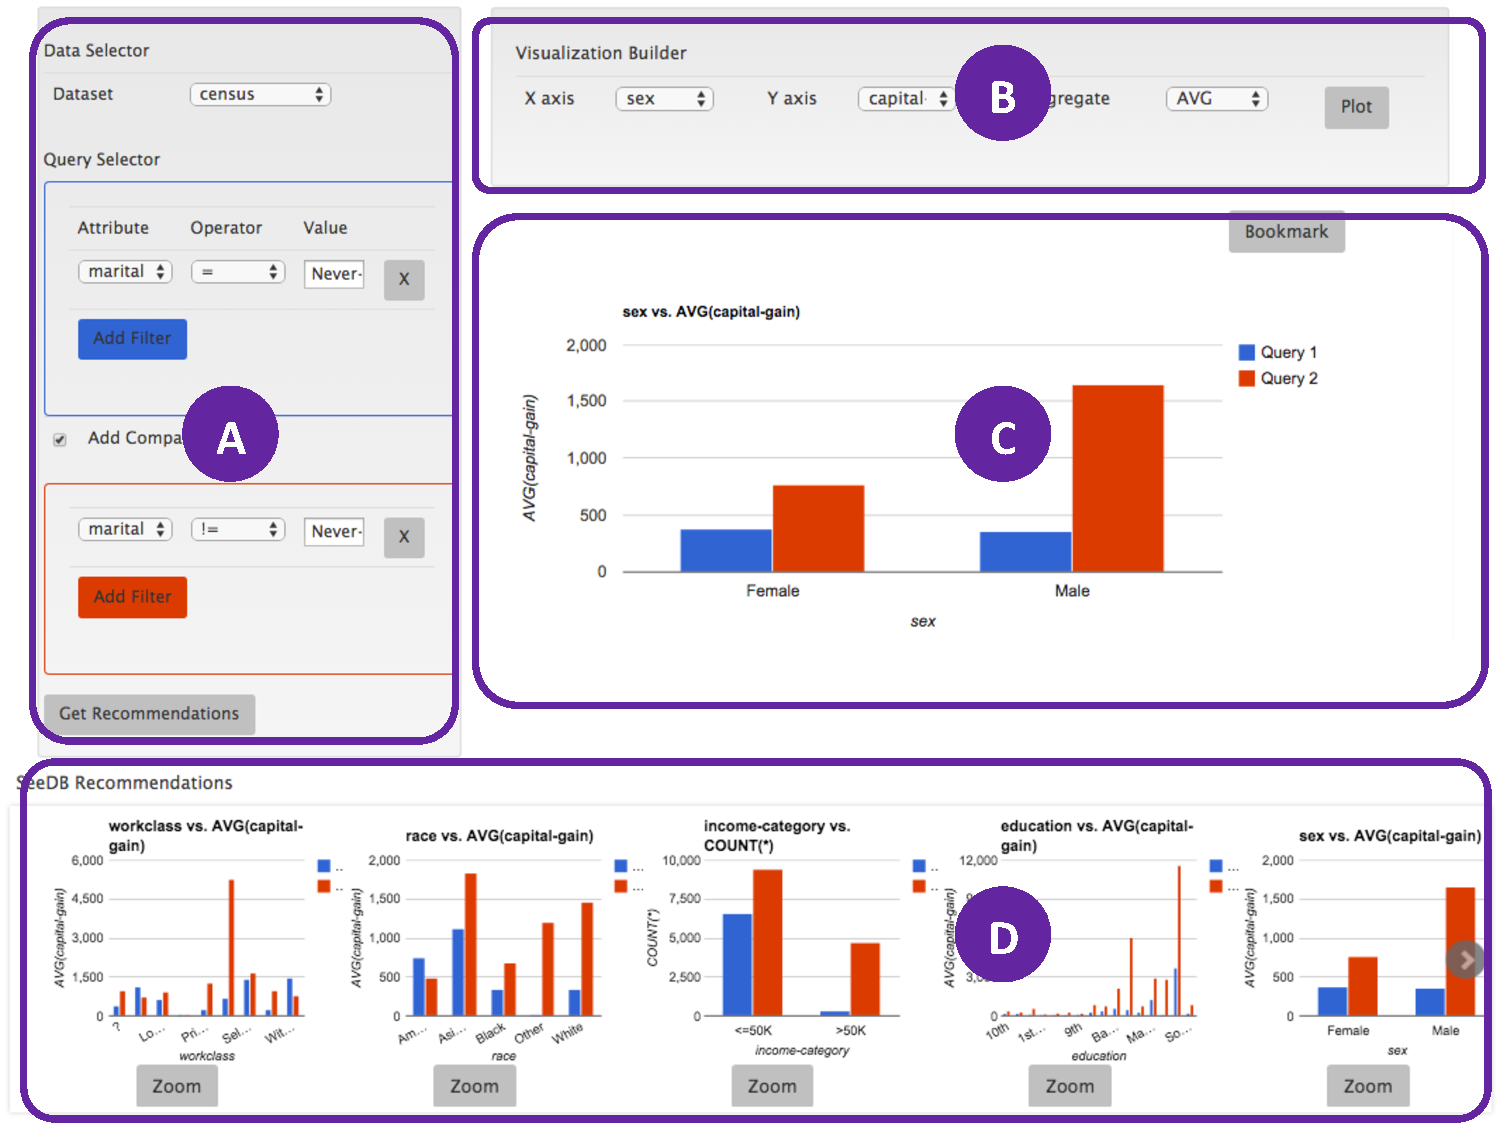
\includegraphics[trim=0mm 0mm 0mm 0mm,
clip=true]{Images/seedb_frontend.pdf}}}}
\caption{\SeeDB Frontend}
\vspace{-20pt}
\label{fig:frontend1}
\end{figure} 


% The optimizer applies multi-query
% optimization 
%  which is responsible for applying multi-query 
% optimization (Section \ref{}) to combine and rewrite DBMS queries 
% corresponding to view in running.
% Next, the execution engine issues optimized queries to the underlying DBMS
% and performs post-processing to compute results for individual views.
% Results from the execution engine are then fed to the pruner which leverages
% view pruning techniques to discard low-utility views.
% The set of views that pass muster with the pruner re-enter the optimizer for
% the next phase of execution.
% Once \SeeDB has identified the top views, the results are returned to the client 
% where \SeeDB frontend generates and displays the recommended visualizations.

% the view generator module queries the system metadata for table sizes, 
% column types, and correlations between column values. 
% It then uses this metadata and the incoming query to remove redundant aggregate views and generate ``stubs'' for the remaining aggregate views.
% The view stubs are then passed to the execution engine which is responsible 
% executing the aggregate views and performing run-time view pruning to identify
% high-utility views.
% To execute aggregate views, the execution engine optimizes the set of aggregate
% views, turns view stubs into SQL queries, and uses the underlying DBMS to efficiently execute the aggregate queries. \mpv{Fix sentence}.
% Once the \SeeDB server has executed the aggregate views and identified the top-k
% views, the data underlying top views is sent to the client where \SeeDB frontend 
% generates and displays the recommended visualizations.

% However, in this work, for ease of development and testing, we built 
% \SeeDB as a standalone end-to-end system that allows users to pose 
% arbitrary queries over data and obtain recommended visualizations.

% The standalone version of \SeeDB\ is comprised of two main components: 
% a light-weight client that is 
% used to issue queries, display recommended visualizations, and allow basic 
% interactions with visualizations; 
% and a server used to generate candidate
% aggregate views, execute
% them over data and identify the aggregate views with highest utility. 
% Figure \ref{fig:sys-arch} depicts the architecture of our system.
% Once the analyst chooses the data of interest (by issuing a query $Q$), the
% client makes a call to the backend for visualization recommendations for $Q$.
% Aggregate view stubs are essentially more elaborate triples of the form $(a, m, f)$ as discussed in Section \ref{sec:problem_statement}. 


% The generated aggregate view stubs are then sent to the execution engine
% responsible for querying the underlying data, evaluating the utility of each
% candidate view, and identifying the top views of interest. 

% Figure \ref{fig:frontend1} shows the \SeeDB client in action; including the supported mechanisms to specify an input query 
% and the visualizations generated by a sample query. 

% In the backend, the view generator module queries the system metadata for table sizes, 
% column types, and correlations between column values. 
% It then uses this metadata and the incoming query to remove redundant aggregate views and generate ``stubs'' for the remaining aggregate views. 
% Aggregate view stubs are essentially more elaborate triples of the form $(a, m, f)$ as
% discussed in Section \ref{sec:problem_statement}. 
% The generated aggregate view stubs are then sent to the execution engine
% responsible for querying the underlying data, evaluating the utility of each
% candidate view, and identifying the top views of interest. 
% Once the \SeeDB\ backend has identified the best aggregate views, the \SeeDB\
% client generates and displays recommended visualizations based on these views.
% Figure \ref{fig:frontend1} shows the \SeeDB client in action; including the supported mechanisms to specify an input query 
% and the visualizations generated by a sample query. 



% In this paper, we build the execution engine in three stages. 
% In the first stage \mpv{better word?}, we implement \SeeDB as a layer on top of the database system and apply traditional multi-query optimization 
% techniques to see how far we can push existing relational databases to support a \SeeDB-type workload.
% While we obtain resonable performance for small datasets, we find the optimizations are insufficient to support large datasets \mpv{quantify?}.
% Therefore, next, we develop a set of pruning techniques that can use running estimates of utility to rapidly prune low-utility views. 
% By reducing the number of views evaluated, these techniques reduce overall latency and also allow \SeeDB to return results without processing the entire dataset.
% We implement these pruning strategies in a simple shared scan system to test the efficacy of our techniques.
% Finally, we build a hybrid execution engine that combines our pruning strategies with the performance optimizations of the DBMS-backed execution engine,
% thus giving us the best of both worlds. 

% In this paper, we explore two distinct implementations of the \SeeDB\ execution
% engine. 
% Our first implementation draws upon traditional multi-query optimization~\cite{}
% and OLAP literature~\cite{} to implement \SeeDB\ as a wrapper
% on top of a database system. \mpv{These techniques are usually inside the DBMS, 
% we are using them outside?}
% The goal of this implementation is to study how far 

% While we obtain reasonable performance by employing well-known optimizations, we find that 
% operating through the SQL interface limits the performance we can obtain.
% Therefore, we next built a custom execution engine that completely shares query scans between
% all views and uses heuristics to rapidly prune low-utility views.
% These techniques allow us to perform only a single pass over the data
% and rapidly identify top visualizations. \mpv{Incorp into DB?}
% However, existing systems do not provide a good means to share scans between
% queries or to access intermediate results during scans.
% As a result, optimization opportunities are limited.
% To overcome the constraints of existing database systems, we implement a
% simple, custom Execution Engine for \SeeDB\ optimized to share scans
% across all views and perform pruning based on intermediate results. 
% In an ideal solution, shared scans and pruning would be implemented inside the
% database; however, for the purpose of this work, we implement the \SeeDB\
% execution engine as a standalone proof-of-concept with a brief discussion of how
% the \SeeDB\ engine could be made part of a DBMS. \mpv{need to add this discussion 
% somewhere}

% Next we briefly examine the \SeeDB client and then describe the execution engines
% in detail.

% In the DBMS-based execution engine (Section \ref{}), the view stubs are passed
% through the optimizer that identifies the best ways to combine the queries to minimize
% execution time.
% Once the views have been optimized, the views are rewritten as SQL queries and
% executed against the underlying database. 
% The results of these queries are
% processed to update the view stubs and compute view utility. 
% Once all the queries have been processed, the top-k views are returned to the
% frontend.
% 
% In the main-memory execution engine, \SeeDB\ makes a single pass through the
% data (either read from disk or already present in memory) and keeps running
% estimates of utility for each of the views stubs obtained from the View
% Generator. 
% As the engine processes more of the data, the utility estimates become more
% accurate and \SeeDB\ uses various pruning heuristics to prune out views on the fly.
% By the time the full data has been processed, \SeeDB\ has identified the top-k
% views with the largest utility that are then returned to the frontend.



%!TEX root = demo-paper.tex
\vspace{-2mm}
\section{Demo Walkthrough}
\label{sec:demo-walkthrough}
 
We propose to demonstrate the functionality of \SeeDB\ through hands-on
interaction with a variety of datasets. Our goals are two fold: (1) demonstrate
the utility of \SeeDB\ in surfacing interesting trends for a query
and (2) demonstrate that we can return high quality views efficiently for
a range of datasets. We will use four different datasets in our demonstration:

\begin{denselist}
  \item {\bf Store Orders dataset}~\cite{superstore}: This dataset is
    often used by Tableau~\cite{tableau} as a canonical dataset for
    business intelligence applications. It consists of information
    about orders placed in a store including products, prices, ship
    dates, geographical information, and profits. Interesting trends in
    this dataset have been very well studied, and attendees will use
    \SeeDB\ to quickly re-identify these trends. 
    %This dataset will also
    %enable us to demonstrate how \SeeDB can correctly deal with
    %numeric, categorical, and geographic data.
  \item {\bf Election Contribution dataset}~\cite{election_data}: This
  is an example of a dataset typically analyzed by
    non-expert data analysts like journalists or historians. With this
    dataset, we demonstrate how non-experts can use \SeeDB\ to quickly
    arrive at interesting visualizations.
  \item {\bf Medical dataset}~\cite{mimic}: This real-world dataset exemplifies
  a dataset that a clinical researcher might use. The schema of the dataset is
  significantly complex and it is of larger size.  
    \item {\bf Synthetic data:} We provide a set of synthetic datasets with
    varying sizes, number of attributes, and data distributions to help
    attendees evaluate \SeeDB\ performance on diverse datasets.
\end{denselist}

\stitle {Scenario 1: Demonstrating Utility.} Attendees are provided with three
diverse, real-world datasets to explore using \SeeDB. For each dataset,
attendees can issue ad-hoc or pre-formulated queries to \SeeDB. \SeeDB\ will
then intelligently explore the view space and optimize query execution to return the
most interesting visualizations with low latency. Attendees can examine the
returned queries visually, view the associated metadata, and perform
drill-downs. To aid the evaluation of visualizations, the demo system will 
be configured to also show the user ``bad'' views (views with low utility) that were not selected
by \SeeDB.
Similarly, we provide pre-selected queries (and
previously known information about their results) to allow attendees to
confirm that \SeeDB\ does indeed reproduce known information about these
queries. Attendees will also be able to experiment with a
variety of distance metrics for computing utility and observe the effects on the
resulting views.

% \stitle{Demonstrating Utility:} To show the utility of \SeeDB\ in a real-world
% scenario, we will provide conference attendees three diverse datasets that they
% can explore and interact with. Attendees can pose ad-hoc or pre-selected queries
% on various datasets and evaluate the visualizations returned. The
% evaluation is based on whether the visualizations surface ``interesting''
% aspects of the queried data and whether the right visualizations have been
% selected. To aid the evaluation of visualizations, the demo version of \SeeDB\
% will have the option of showing ``bad'' visualizations too, i.e. visualizations
% that were predicted to have low utility.  The attendees will also have the option of
% trying various utility metrics as described in Section
% \ref{sec:problem_statement}. The demo datasets will include:

\stitle{Scenario 2: Demonstrating Performance and Optimizations.} This scenario
will use an enhanced user interface and synthetic datasets mentioned above.
Attendees will be able to easily experiment with a range of synthetic datasets and input
queries by adjusting various ``knobs'' such as data size, number of attributes, and
data distribution. In addition, attendees will also be able to select the
optimizations that \SeeDB\ applies and observe the effect on response times and
accuracy.

Thus, through our demonstration of \SeeDB\, we seek to illustrate that (a) it is
possible to automate labor-intensive parts of data analysis, (b) aggregate
and grouping-based views are a powerful means to identify interesting trends
in data, and (c) the right set of optimizations can enable real-time data
analysis of large datasets.

\eat{
We propose to demonstrate the functionality of the SeeDB system by means of
analyzing three diverse datasets of practical importance. Users will be able to
explore each of these datasets in real-time by using SeeDB to formulate
queries and find interesting trends in the underlying dataset. Specifically, we
will use the following datasets for demonstration purposes:

\begin{itemize}
  \item {\bf Store Orders dataset}: This is a canonical dataset used in business
  intelligence applications. It consists of information about orders placed in a
  store including products, prices, ship dates, geographical information,
  profits etc. The dataset is well known for its interesting trends and
  richness of various data types. It will show off SeeDB capabilities to
  correctly identify diverse trends in the data and the ability to deal with
  numeric, categorical, time series and geographic data.
  \item {\bf Election Contribution dataset}: This dataset is a great example of
  the kind of data and analysis that must be done by potential users like
  journalists who are not data analysts by trade but often need to find
  interesting trends in datasets. As a result, this use case will help the
  audience guage the intuitiveness of the user interface, ease of use and fast
  response times.
  \item {\bf Medical dataset:} This dataset is an example of a dataset that a
  researcher (here, a clinical researcher) might use over the course of his/her
  work. This data has a schema that is more complex than the the election
  or store one, and is of larger size too. Since this data is usually analyzed
  by experts, in addition to fast provision of insights, the user also cares about
  flexiblity and ``expert'' operations on this data such as statistical
  information, accuracy of visualizations, drill-downs etc.
\end{itemize}

We envision the demonstration workflow to be as follows: The user selects one of
the three dataset from above for analysis. He/she formulates a selection query
using the SeeDB query builder or by using ready-made queries (e.g. selecting
outliers in a column etc.) and submits the query to SeeDB. SeeDB then searches
through the entire space of possible views using techniques and heuristics
described in Section \ref{optimizations} and returns the top-{\it k} views it
considers most interesting. The SeeDB frontend then visualizes the top-{it k} views and
presents them to the user. The user can interact with each of these views and
perform further exploration through operations such as drill-downs (graphically
selecting subsets of data), comparisons of multiple views etc. The user will
also be able to experiment with the effect of choosing different utility metrics
and optimization strategies described in Section \ref{}.
}
  
\vspace{-2mm}
{\scriptsize
\bibliographystyle{abbrv}
\bibliography{visubib}
}


\end{document}


